\documentclass[10pt,conference,compsocconf]{IEEEtran}
\usepackage[usenames,dvipsnames]{color}
%\usepackage[english]{babel}
\usepackage{tabularx}
\usepackage{soul}
\usepackage{xparse}
\usepackage{listings}
%\usepackage[normalem]{ulem}



%%%%%%%%%%%%%%%
% Show a list of items "todo" or "done" 
% USAGE: 
% \begin{todolist} 
% 	\todo Something not finished
% 	\done Something finished
% \end{todolist} 
\newenvironment{todolist}{%
  \begin{list}{}{}% whatever you want the list to be
  \let\olditem\item
  \renewcommand\item{\olditem \textcolor{red}{(TODO)}: }
  \newcommand\todo{\olditem \textcolor{red}{(TODO)}: }
   \newcommand\done{\olditem \textcolor{ForestGreen}{(DONE)}: }
}{%
  \end{list}
} 
%%%%%%%%%%%%%%%

%%%%%%%%%%%%%%%
% Show a Author's Note
% USAGE: 
% \incomplete[Optional footnote message to further clarify note]{The text which is currently not finished}
\DeclareDocumentCommand \incomplete{ o m }
{%
\IfNoValueTF {#1}
{\textcolor{red}{Incomplete: \ul{#2}}} 
{\textcolor{red}{Incomplete: \ul{#2}}\footnote{Comment: #1}}%
}
%%%%%%%%%%%%%%%



%%%%%%%%%%%%%%%
% Show a Author's Note
% USAGE: 
% \authnote[Optional footnote message to further clarify note]{The note to your readers}
\DeclareDocumentCommand \authnote { o m }
{%
\IfNoValueTF {#1}
{\textcolor{blue}{Author's Note: \ul{#2}}} 
{\textcolor{blue}{Author's Note: \ul{#2}}\footnote{Comment: #1}}%
}
%%%%%%%%%%%%%%%



%%%%%%%%%%%%%%%
% Strike out text that doesn't belong in the paper
% USAGE: 
% \strike[Optional footnote to state why it doesn't belong]{Text to strike out}
\DeclareDocumentCommand \strike { o m }
{%
\setstcolor{Red}
\IfNoValueTF {#1}
{\textcolor{Gray}{\st{#2}}} 
{\textcolor{Gray}{\st{#2}}\footnote{Comment: #1}}%
}
%%%%%%%%%%%%%%%

\definecolor{light-gray}{gray}{0.95}

\newcommand{\cbox}[3]{
\ \\
\fcolorbox{#1}{#2}{
\parbox{\textwidth}{
#3
}
}
}

% Setup an environment similar to verbatim but which will highlight any bash commands we have
\lstnewenvironment{unixcmds}[0]
{
%\lstset{language=bash,frame=shadowbox,rulesepcolor=\color{blue}}
\lstset{ %
language=sh,		% Language
basicstyle=\ttfamily,
backgroundcolor=\color{light-gray}, 
rulecolor=\color{blue},
%frame=tb, 
columns=fullflexible,
%framexrightmargin=-.2\textwidth,
linewidth=0.8\textwidth,
breaklines=true,
%prebreak=/, 
  prebreak = \raisebox{0ex}[0ex][0ex]{\ensuremath{\hookleftarrow}},
%basicstyle=\footnotesize,       % the size of the fonts that are used for the code
%numbers=left,                   % where to put the line-numbers
%numberstyle=\footnotesize,      % the size of the fonts that are used for the line-numbers
%stepnumber=2,                   % the step between two line-numbers. If it's 1 each line 
                                % will be numbered
%numbersep=5pt,                  % how far the line-numbers are from the code
showspaces=false,               % show spaces adding particular underscores
showstringspaces=false,         % underline spaces within strings
showtabs=false,                 % show tabs within strings adding particular underscores
frame=single,	                % adds a frame around the code
tabsize=2,	                % sets default tabsize to 2 spaces
captionpos=b,                   % sets the caption-position to bottom
breakatwhitespace=false,        % sets if automatic breaks should only happen at whitespace
}
} { }

% Setup an environment similar to verbatim but which will highlight any bash commands we have
\lstnewenvironment{cppcode}[1]
{
%\lstset{language=bash,frame=shadowbox,rulesepcolor=\color{blue}}
\lstset{ %
	backgroundcolor=\color{light-gray}, 
	rulecolor=\color[rgb]{0.133,0.545,0.133},
	tabsize=4,
	language=[GNU]C++,
%	basicstyle=\ttfamily,
        basicstyle=\scriptsize,
        upquote=true,
        aboveskip={1.5\baselineskip},
        columns=fullflexible,
        %framexrightmargin=-.1\textwidth,
       %framexleftmargin=6mm,
        showstringspaces=false,
        extendedchars=true,
        breaklines=true,
        prebreak = \raisebox{0ex}[0ex][0ex]{\ensuremath{\hookleftarrow}},
        frame=single,
        showtabs=false,
        showspaces=false,
        showstringspaces=false,
        numbers=left,                   % where to put the line-numbers
	numberstyle=\footnotesize,      % the size of the fonts that are used for the line-numbers
	stepnumber=4,                   % the step between two line-numbers. If it's 1 each line 
                                % will be numbered
	firstnumber=#1,
         numbersep=5pt,                  % how far the line-numbers are from the code
        identifierstyle=\ttfamily,
        keywordstyle=\color[rgb]{0,0,1},
        commentstyle=\color[rgb]{0.133,0.545,0.133},
        stringstyle=\color[rgb]{0.627,0.126,0.941},
}
} { }

% Setup an environment similar to verbatim but which will highlight any bash commands we have
\lstnewenvironment{mcode}[1]
{
\lstset{ %
	backgroundcolor=\color{light-gray}, 
	rulecolor=\color[rgb]{0.133,0.545,0.133},
	tabsize=4,
	language=Matlab,
%	basicstyle=\ttfamily,
        basicstyle=\scriptsize,
        upquote=true,
        aboveskip={1.5\baselineskip},
        columns=fullflexible,
        %framexrightmargin=-.1\textwidth,
       %framexleftmargin=6mm,
        showstringspaces=false,
        extendedchars=true,
        breaklines=true,
        prebreak = \raisebox{0ex}[0ex][0ex]{\ensuremath{\hookleftarrow}},
        frame=single,
        showtabs=false,
        showspaces=false,
        showstringspaces=false,
        numbers=left,                   % where to put the line-numbers
	numberstyle=\footnotesize,      % the size of the fonts that are used for the line-numbers
	stepnumber=4,                   % the step between two line-numbers. If it's 1 each line 
                                % will be numbered
	firstnumber=#1,
         numbersep=5pt,                  % how far the line-numbers are from the code
        identifierstyle=\ttfamily,
        keywordstyle=\color[rgb]{0,0,1},
        commentstyle=\color[rgb]{0.133,0.545,0.133},
        stringstyle=\color[rgb]{0.627,0.126,0.941},
}
} { }

\newcommand{\inputmcode}[1]{%
\lstset{ %
	backgroundcolor=\color{light-gray},  %
	rulecolor=\color[rgb]{0.133,0.545,0.133}, %
	tabsize=4, %
	language=Matlab, %
%	basicstyle=\ttfamily,
        basicstyle=\scriptsize, %
        %        upquote=true,
        aboveskip={1.5\baselineskip}, %
        columns=fullflexible, %
        %framexrightmargin=-.1\textwidth,
       %framexleftmargin=6mm,
        showstringspaces=false, %
        extendedchars=true, %
        breaklines=true, %
        prebreak = \raisebox{0ex}[0ex][0ex]{\ensuremath{\hookleftarrow}}, %
        frame=single, %
        showtabs=false, %
        showspaces=false, %
        showstringspaces=false,%
        numbers=left,                   % where to put the line-numbers
	numberstyle=\footnotesize,      % the size of the fonts that are used for the line-numbers
	stepnumber=4,                   % the step between two line-numbers. If it's 1 each line 
                                % will be numbered
         numbersep=5pt,                  % how far the line-numbers are from the code
        identifierstyle=\ttfamily, %
        keywordstyle=\color[rgb]{0,0,1}, %
        commentstyle=\color[rgb]{0.133,0.545,0.133}, %
        stringstyle=\color[rgb]{0.627,0.126,0.941} %
}
\lstinputlisting{#1}%
}

%\lstset{ %
%	backgroundcolor=\color{light-gray}, 
%	rulecolor=\color[rgb]{0.133,0.545,0.133},
%	tabsize=4,
%	language=Matlab,
%%	basicstyle=\ttfamily,
%        basicstyle=\scriptsize,
%        upquote=true,
%        aboveskip={1.5\baselineskip},
%        columns=fullflexible,
%        %framexrightmargin=-.1\textwidth,
%       %framexleftmargin=6mm,
%        showstringspaces=false,
%        extendedchars=true,
%        breaklines=true,
%        prebreak = \raisebox{0ex}[0ex][0ex]{\ensuremath{\hookleftarrow}},
%        frame=single,
%        showtabs=false,
%        showspaces=false,
%        showstringspaces=false,
%        numbers=left,                   % where to put the line-numbers
%	numberstyle=\footnotesize,      % the size of the fonts that are used for the line-numbers
%	stepnumber=4,                   % the step between two line-numbers. If it's 1 each line 
%                                % will be numbered
%	firstnumber=#1,
%         numbersep=5pt,                  % how far the line-numbers are from the code
%        identifierstyle=\ttfamily,
%        keywordstyle=\color[rgb]{0,0,1},
%        commentstyle=\color[rgb]{0.133,0.545,0.133},
%        stringstyle=\color[rgb]{0.627,0.126,0.941},
%}


\newcommand{\Laplacian}[1]{\nabla^2 #1}

% set of all nodes received and contained on GPU
\newcommand{\setAllNodes}[0]{\mathcal{G}}
% set of stencil centers on GPU
\newcommand{\setCenters}[0]{\mathcal{Q}}
% set of stencil centers with nodes in \setDepend
\newcommand{\setBoundary}[0]{\mathcal{B}}
% set of nodes received by other GPUs
\newcommand{\setDepend}[0]{\mathcal{R}}
% set of nodes sent to other GPUs
\newcommand{\setProvide}[0]{\mathcal{O}}


\newcommand{\toprule}[0]{\hline}
\newcommand{\midrule}[0]{\hline\hline}
\newcommand{\bottomrule}[0]{\hline}

\newcolumntype{C}{>{\centering\arraybackslash}b{1in}}
\newcolumntype{L}{>{\flushleft\arraybackslash}b{1.5in}}
\newcolumntype{R}{>{\flushright\arraybackslash}b{1.5in}}
\newcolumntype{D}{>{\flushright\arraybackslash}b{2.0in}}
\newcolumntype{E}{>{\flushright\arraybackslash}b{1.0in}}

\DeclareSymbolFont{AMSb}{U}{msb}{m}{n}
\DeclareMathSymbol{\N}{\mathbin}{AMSb}{"4E}
\DeclareMathSymbol{\Z}{\mathbin}{AMSb}{"5A}
\DeclareMathSymbol{\R}{\mathbin}{AMSb}{"52}
\DeclareMathSymbol{\Q}{\mathbin}{AMSb}{"51}
\DeclareMathSymbol{\PP}{\mathbin}{AMSb}{"50}
\DeclareMathSymbol{\I}{\mathbin}{AMSb}{"49}
%\DeclareMathSymbol{\C}{\mathbin}{AMSb}{"43}

%%%%%% VECTOR NORM: %%%%%%%
\newcommand{\vectornorm}[1]{\left|\left|#1\right|\right|}
\newcommand{\vnorm}[1]{\left|\left|#1\right|\right|}
\newcommand{\by}[0]{\times}
\newcommand{\vect}[1]{\mathbf{#1}}
%\newcommand{\mat}[1]{\mathbf{#1}} 

%\renewcommand{\vec}[1]{ \textbf{#1} }
%%%%%%%%%%%%%%%%%%%%%%

%%%%%%% THM, COR, DEF %%%%%%%
%\newtheorem{theorem}{Theorem}[section]
%\newtheorem{lemma}[theorem]{Lemma}
%\newtheorem{proposition}[theorem]{Proposition}
%\newtheorem{corollary}[theorem]{Corollary}
%\newenvironment{proof}[1][Proof]{\begin{trivlist}
%\item[\hskip \labelsep {\bfseries #1}]}{\end{trivlist}}
%\newenvironment{definition}[1][Definition]{\begin{trivlist}
%\item[\hskip \labelsep {\bfseries #1}]}{\end{trivlist}}
%\newenvironment{example}[1][Example]{\begin{trivlist}
%\item[\hskip \labelsep {\bfseries #1}]}{\end{trivlist}}
%\newenvironment{remark}[1][Remark]{\begin{trivlist}
%\item[\hskip \labelsep {\bfseries #1}]}{\end{trivlist}}
%\newcommand{\qed}{\nobreak \ifvmode \relax \else
%      \ifdim\lastskip<1.5em \hskip-\lastskip
%      \hskip1.5em plus0em minus0.5em \fi \nobreak
%      \vrule height0.75em width0.5em depth0.25em\fi}
%%%%%%%%%%%%%%%%%%%%%%

%
%\usepackage[algochapter]{algorithm2e}
%\usepackage[usenames]{color}
% colors to show the corrections
\newcommand{\red}[1]{\textbf{\textcolor{red}{#1}}}
\newcommand{\blue}[1]{\textbf{\textcolor{blue}{#1}}}
\newcommand{\cyan}[1]{\textbf{\textcolor{cyan}{#1}}}
\newcommand{\green}[1]{\textbf{\textcolor{green}{#1}}}
\newcommand{\magenta}[1]{\textbf{\textcolor{magenta}{#1}}}
\newcommand{\orange}[1]{\textbf{\textcolor{orange}{#1}}}
%%%%%%%%%% DK DK
% comments between authors
\newcommand{\toall}[1]{\textbf{\green{@@@ All: #1 @@@}}}
\newcommand{\toevan}[1]{\textbf{\red{*** Evan: #1 ***}}}
%\newcommand{\toevan}[1]{}  % USE FOR FINAL VERSION
\newcommand{\toe}[1]{\textbf{\red{*** Evan: #1 ***}}}
%\newcommand{\toe}[1]{\textbf{\red{*** Evan: #1 ***}}}
\newcommand{\tog}[1]{\textbf{\blue{*** Gordon: #1 ***}}}
%\newcommand{\togordon}[1]{\textbf{\blue{*** Gordon: #1 ***}}}

\renewcommand{\ge}[3]{{\textcolor{blue}{\strike{#1} #2}}\red{(#3)}}
%\renewcommand{\ge}[3]{{\textcolor{blue}{*** \textbf{Gordon:}\strike{#1} #2 ***}}\red{(#3)}}

\newcommand{\gea}[3]{{\textcolor{blue}{\textbf{(Accepted) Gordon:}\strike{#1} #2}}\red{(#3)}}
%\newcommand{\gea}[3]{{\textcolor{blue}{*** \textbf{(Accepted) Gordon:}\strike{#1} #2 ***}}\red{(#3)}}

\newcommand{\eb}[3]{{\textcolor{ForestGreen}{\strike{#1} #2}}\red{(#3)}}
%\newcommand{\eb}[3]{{\textcolor{ForestGreen}{*** \textbf{Evan:}\strike{#1} #2 ***}}\red{(#3)}}

%\def\ge#1#2#3{}{\textbf{\blue{*** Gordon: #2 ***}}}{(#3)}
\newcommand{\gee}[1]{{\bf{\blue{{\em #1}}}}}
\newcommand{\old}[1]{}
\newcommand{\del}[1]{***#1*** }



% \DeclareMathOperator{\Sample}{Sample}
%\let\vaccent=\v % rename builtin command \v{} to \vaccent{}
%\renewcommand{\vec}[1]{\ensuremath{\mathbf{#1}}} % for vectors
\newcommand{\gv}[1]{\ensuremath{\mbox{\boldmath$ #1 $}}} 
% for vectors of Greek letters
\newcommand{\uv}[1]{\ensuremath{\mathbf{\hat{#1}}}} % for unit vector
\newcommand{\abs}[1]{\left| #1 \right|} % for absolute value
\newcommand{\avg}[1]{\left< #1 \right>} % for average
\let\underdot=\d % rename builtin command \d{} to \underdot{}
\renewcommand{\d}[2]{\frac{d #1}{d #2}} % for derivatives
\newcommand{\dd}[2]{\frac{d^2 #1}{d #2^2}} % for double derivatives
\newcommand{\pd}[2]{\frac{\partial #1}{\partial #2}} 
% for partial derivatives
\newcommand{\pdd}[2]{\frac{\partial^2 #1}{\partial #2^2}} 
\newcommand{\pdda}[3]{\frac{\partial^2 #1}{\partial #2 \partial #3}} 
% for double partial derivatives
\newcommand{\pdc}[3]{\left( \frac{\partial #1}{\partial #2}
 \right)_{#3}} % for thermodynamic partial derivatives
\newcommand{\ket}[1]{\left| #1 \right>} % for Dirac bras
\newcommand{\bra}[1]{\left< #1 \right|} % for Dirac kets
\newcommand{\braket}[2]{\left< #1 \vphantom{#2} \right|
 \left. #2 \vphantom{#1} \right>} % for Dirac brackets
\newcommand{\matrixel}[3]{\left< #1 \vphantom{#2#3} \right|
 #2 \left| #3 \vphantom{#1#2} \right>} % for Dirac matrix elements
\newcommand{\grad}[1]{\gv{\nabla} #1} % for gradient
\let\divsymb=\div % rename builtin command \div to \divsymb
\renewcommand{\div}[1]{\gv{\nabla} \cdot #1} % for divergence
\newcommand{\curl}[1]{\gv{\nabla} \times #1} % for curl
\let\baraccent=\= % rename builtin command \= to \baraccent
\renewcommand{\=}[1]{\stackrel{#1}{=}} % for putting numbers above =
\newcommand{\diffop}[1]{\mathcal{L}#1}
\newcommand{\boundop}[1]{\mathcal{B}#1}
\newcommand{\rvec}[0]{{\bf r}}

\newcommand{\Interior}[0]{\Omega}
\newcommand{\domain}[0]{\Omega}
%\newcommand{\Boundary}[0]{\partial \Omega}
\newcommand{\Boundary}[0]{\Gamma}

\newcommand{\on}[1]{\hskip1.5em \textrm{ on } #1}

\newcommand{\gemm}{\texttt{GEMM}}
\newcommand{\trmm}{\texttt{TRMM}}
\newcommand{\gesvd}{\texttt{GESVD}}
\newcommand{\geqrf}{\texttt{GEQRF}}


\newcommand{\minitab}[2][l]{\begin{tabular}{#1}#2\end{tabular}}
\newcommand{\comm}[1]{\textcolor{red}{\textit{#1}}}

\newcommand{\nfrac}[2]{
\nicefrac{#1}{#2}
%\frac{#1}{#2}
}
 % color is defined in macros or misc_mac
% Rename  this file          misc_mac.tex
%----------------------------------------------------------------------
%%%%%%%%%%%%%%%%%%%%%%%%%%%%%%%%%%%%%%%%%%%%%%%%%%%%%%%%%%%%%%%%%%%%%%%%%%%%%%%
%
%	Math Symbols   Math Symbols   Math Symbols   Math Symbols   
%
%%%%%%%%%%%%%%%%%%%%%%%%%%%%%%%%%%%%%%%%%%%%%%%%%%%%%%%%%%%%%%%%%%%%%%%%%%%%%%%
\def\pmb#1{\setbox0=\hbox{$#1$}%
	\kern-.025em\copy0\kern-\wd0
	\kern.05em\copy0\kern-\wd0
	\kern-.025em\raise.0433em\box0}
\def\pmbf#1{\pmb#1}
\def\bfg#1{\pmb#1}

% BETTER VALUES FOR AUTOMATIC FIGURE PLACEMENT THAN THOSE PROVIDED BY 
% LATEX DEFAULTS.

\renewcommand{\textfloatsep}{1ex}
\renewcommand{\floatpagefraction}{0.9}
\renewcommand{\intextsep}{1ex}
\renewcommand{\topfraction}{.9}
\renewcommand{\bottomfraction}{.9}
\renewcommand{\textfraction}{.1}

% #1  position of floating figure (h|t|b|p)
% #1  EPS postscript file
% #2  size
% #3  caption

%usage of newfig:
%  \newfig{file.ps}{3in}{Fig1: this is a figure}

\input{epsf}
\def\newfig#1#2#3#4{
  \begin{figure}[htbp]
  \centering
  \vspace{1ex}
   \includegraphics[width=#2]{#1}
  %\setlength{\epsfxsize}{#2}
  \vspace{-.1in}\caption{\small #3}\break\vspace{.2in}
  \label{#4}
  \end{figure}
}

\def\herefig#1#2#3#4{
  \begin{figure}[h]
  \centering
  \vspace{1ex}
   \includegraphics[width=#2\textwidth]{#1}
  %\setlength{\epsfxsize}{#2}
  \vspace{-.1in}\caption{\small #3}\break\vspace{.2in}
  \label{#4}
  \end{figure}
}


%usage of newfigtwo: 2 figures, vertically stacked
% \newfig
%	{file1.ps}
%	{file2.ps}
%	{width}
%	{vertical space}
%	{Caption}

\def\newfigtwo#1#2#3#4#5{
  \begin{figure}[htbp]
  \vspace{1ex}
  \setlength{\epsfxsize}{#3}
  \centerline{\epsfbox{#1}}
  \vspace{#4}
  \setlength{\epsfxsize}{#3}
  \centerline{\epsfbox{#2}}
  \vspace{-.1in}\caption{\small #5}\break\vspace{.2in}
  \label{#1}
  \end{figure}
}

\def\newfigh#1#2#3#4{  % add height specification
  \begin{figure}[htbp]
  \vspace{1ex}
  \setlength{\epsfxsize}{#2}
  \setlength{\epsfysize}{#4}
  \centerline{\epsfbox{#1}}
  \vspace{-.1in}\caption{\small #3}\break\vspace{.2in}
  \label{#1}
  \end{figure}
}

\def\etal{{{\em et~al.\,\,}}}
\def\note#1{\\ =====#1===== \\}
\def\FBOX#1{\ \\ \fbox{\begin{minipage}{5in}#1\end{minipage}}\\ }
\newcount\sectionno     \sectionno=0
\newcount\eqnum         \eqnum=0
\def\addeqno{\global\advance \eqnum by  1 }
\def\subeqno{\global\advance \eqnum by -1 }
%\def\eqn{\addeqno \eqno \hbox{(\number\sectionno.\number\eqnum)} }

\def\tildetilde#1{\tilde{\tilde{#1}}}
\def\barbar#1{\overbar{\overbar{#1}}}

\def\vsp#1{\vspace{#1 ex}}
\def\fpar{\hspace{\parindent}}
%
%  \pf : 2 arguments: numerator and denominator of partial derivative
%
\def\pf#1#2{{\frac{\partial{#1}}{\partial{#2}}}}
\def\pfs#1#2{{\partial_{#2}{#1}}}
\def\pftwo#1#2{{\frac{\partial^2{#1}}{\partial{#2}^2}}}
\def\pfxx#1#2{{\frac{\partial^2{#1}}{\partial{#2}^2}}}
%\def\pfxy#1#2{{\frac{\partial^2{#1}}{\partial{#2}\partial{#3}}}}
\def\pfn#1#2#3{{\frac{\partial^{#1}{#2}}{\partial{#3}^{#1}}}}
\def\df#1#2{{\frac{d{#1}}{d{#2}}}}
\def\dfn#1#2#3{{\frac{d^{#1}{#2}}{d{#3}^{#1}}}}
\def\Dt#1#2{\frac{D#1}{D#2}}
\def\dt#1#2{\frac{d#1}{d#2}}
\def\bld#1{{\bf #1}}
\def\pfp#1#2#3{\pf{}{#3}{\left(\frac{#1}{#2}\right)}}

\def\norm#1{\|#1\|}

%
% Graphic characters  (\dot already defined by TeX/LateX)
%
\def\dash{\rule[1.5pt]{2mm}{.3mm}\HS{.9mm}}
\def\dott{\rule[1.5pt]{.7mm}{.3mm}\HS{.7mm}}
\def\dashline{\dash\dash\dash}
\def\dotline{\dott\dott\dott\dott\dott\dott}
\def\dashdotline{\dash$\cdot$\HS{.9mm}\dash}
\def\solidline{\rule[2pt]{7mm}{.3mm}}
% 
% overcircle
%
\def\ovcircle#1{\buildrel{\circ}\over{#1}}
%\def\below#1#2{\buildrel{#2}\under{#1}}
%\def\above#1#2{\buildrel{#2}\over{#1}}
%
%  big parenthesis and brackets
%
\def\bigpar#1#2{{\left(\frac{#1}{#2}\right)}}
\def\bigbra#1#2{{\left\[\frac{#1}{#2}\right\]}}

\def\Lp{\left(}
\def\Rp{\right)}
\def\Lb{\left[}
\def\Rb{\right]}
\def\Ln{\left\langle}
\def\Rn{\right\rangle}
\def\Ld{\left.}
\def\Rd{\right.}
\def\Lv{\left|}
\def\Rv{\right|}
\def\Lbr{\left|}
\def\Rbr{\right|}
\def\lng{\langle}
\def\rng{\rangle}
\def\Lc{\left\{}
\def\Rc{\right\}}
%%% %

% Cannot be handled by Lyx
%\def\[{{[}}
%\def\]{{]}}

%
\def\eol{\nonumber \\}
\def\eolnonb{\nonumber\\}
\def\eolnb{\\}
\def\nonb{\nonumber}
\def\be{\begin{equation}}
\def\ee{\end{equation}}
\def\BEQNA{\begin{eqnarray}}
\def\EEQNA{\end{eqnarray}}
\def\eqa{&=&}
\def\beqna{\begin{eqnarray}}
\def\eeqna{\end{eqnarray}}
\def\bverb{\begin{verbatim}}
\def\everb{\end{verbatim}}
\def\VERB#1{\bverb #1 \everb}
\def\btbl{\begin{tabular}}
\def\etbl{\end{tabular}}
\def\bmini{\begin{minipage}[t]{5.5in}}
\def\emini{\end{minipage}}
\def\parray#1#2{\left(\!\!\!\begin{array}{#1}#2\end{array}\!\!\!\right)}
\def\barray#1#2{\left[\begin{array}{#1}#2\end{array}\right]}
\def\carray#1#2{\left\{\begin{array}{#1}#2\end{array}\right.}
\def\darray#1#2{\left|\begin{array}{#1}#2\end{array}\right|}

\def\BEGTABLE#1{\begin{table}[hbt]\vspace{2ex}\begin{center}\bmini\centering\btbl{#1}}
\def\ENDTABLE#1#2{\etbl\caption[#1]{#2}\EMINI\end{center}\vspace{2ex}\end{table}}

\def\bfltbl#1{\begin{table}[hbt]\vspace{2ex}\begin{center}\bmini\centering\btbl{#1}}
\def\efltbl#1#2{\etbl\caption[#1]{#2}\emini\end{center}\vspace{2ex}\end{table}}
\def\mcol{\multicolumn}
%
%  label equations with (#)
%
\def\reff#1{(\ref{#1})}
%
%  macros borrowed from viewgraph package
%

\newenvironment{LETTRS}[3]{\begin{letter}{#1}
\input{origin}\opening{Dear #2:}\input{#3}\closing{Sincerely yours,}\end{letter}}{\clearpage}

\newenvironment{VIEW}[1]{{\BC\Huge\bf #1 \EC}\LARGE\VS{.05in}}{\clearpage}

\def\RM#1{\rm{#1\ }}
\def\BV{\begin{VIEW}}
\def\EV{\end{VIEW}}

\def\NI{\noindent}

\def\VS{\vspace*}
\def\HS{\hspace*}
\def\IT{\item}

\def\BARR{\begin{array}}
\def\EARR{\end{array}}

\def\BPARR{\left(\begin{array}}
\def\EPARR{\end{array}\right)}

\def\BDET{\left|\begin{array}}
\def\EDET{\end{array}\right|}

\def\BDF{\begin{definition}}
\def\EDF{\end{definition}}

\def\BSU{\begin{block}{Summary}}
\def\ESU{\end{block}}

\def\BEX{\begin{example}}
\def\EEX{\end{example}}

\def\BTH{\begin{theorem}}
\def\ETH{\end{theorem}}

\def\BCO{\begin{corollary}}
\def\ECO{\end{corollary}}

\def\BPROOF{\begin{proof}}
\def\EPROOF{\end{proof}}

\def\BLM{\begin{lemma}}
\def\ELM{\end{lemma}}

\def\BEQ{\begin{equation}}
\def\EEQ{\end{equation}}

\def\BEQNNB{$$}
\def\EEQNNB{$$}

\def\BE{\begin{enumerate}}
\def\EE{\end{enumerate}}

\def\BD{\begin{description}}
\def\ED{\end{description}}

\def\BI{\begin{itemize}}
\def\EI{\end{itemize}}

\def\BC{\begin{center}}
\def\EC{\end{center}}

\def\BFIG{\begin{figure}}
\def\EFIG{\end{figure}}

\def\BTABB{\begin{tabbing}}
\def\ETABB{\end{tabbing}}

\def\BMINI{\begin{minipage}}
\def\EMINI{\end{minipage}}

\def\BTABLE{\begin{table}}
\def\ETABLE{\end{table}}

\def\BTABUL{\begin{tabular}}
\def\ETABUL{\end{tabular}}

\def\MCOL{\multicolumn}
\def\UL{\underline}
\def\ULL#1{\UL{\UL{#1}}}

\def\BDOC{\begin{document}}
\def\EDOC{\end{document}}

\def\EM#1{{\em #1\/}}
\def\FN{\footnote}

% Courtesy of Ugo Piomelli

\def\latexfig #1 #2 #3 #4 #5 {\ \vfill
\hfill\hbox to 0.05in{\vbox to #3truein{
         \special{psfile="#1" angle=270 hscale=100 
                  hoffset=#4 voffset=#5 vscale=100} }\hfill}
\hfill\vspace{-0.1in}        }

% #1 is the .ps filename
% #2 is not used in the present version
% #3 is the size of the white space left above the caption (in inches)
% #4 is the horizontal offset from some unknown reference point.
%    It is in 1/72 of an inch and is positive to the right.
% #5 is the vertical offset from some unknown reference point.
%    It is in 1/72 of an inch and is positive upwards.


% Rename this file:    setupicase.tex
%----------------------------------------------------------------------
\setlength{\textwidth}{6.5in}
\setlength{\textheight}{9.0in}
\setlength{\topmargin}{-.1875pt}
\setlength{\oddsidemargin}{0pt}
\setlength{\evensidemargin}{0pt}
\setlength{\headsep}{0pt}
\setlength{\parskip}{1ex}
\setlength{\headheight}{0pt}



\def\red#1{\textbf{\textcolor{red}{#1}}}
\def\blue#1{\textbf{\textcolor{blue}{#1}}}
\def\qes#1{{\blue{*** For Erik: #1 ***}}}
\def\es#1{{\blue{*** For Erik: #1 ***}}}
\def\ge#1{{\red{*** For Gordon: #1 ***}}}
\def\ttt#1{{\tt #1}}
\def\bold#1{{\bf #1}}

\usepackage{soul}
\usepackage{xspace}
\usepackage{color} 
\definecolor{darkgreen}{rgb}{0,0.5,0}
\usepackage[colorlinks=true,% 
  linkcolor=red,% 
  citecolor=darkgreen,%
  urlcolor=blue]{hyperref}

\usepackage{listings}


\newcommand{\todo}[1]{{\color{red}\textbf{\hl{#1}}\xspace}}

\def\qes#1{}
\def\es#1{}
%\def\ge#1{}
%\usepackage{morefloats}

\newcommand{\ceil}[1]{\left\lceil#1\right\rceil}
\newcommand{\floor}[1]{\left\lfloor#1\right\rfloor}

\usepackage{amsmath}
\usepackage{amssymb}


\usepackage[pdftex]{graphicx}
\usepackage{subfigure}
%\usepackage{fixltx2e}
\usepackage{url}
\hyphenation{op-tical net-works semi-conduc-tor}


\begin{document}
\title{Acceleration of Derivative Calculations with Application to Radial Basis Function --
Finite-Differences on the MIC Architecture}
%\title{Sparse Matrix Vector Multiplication with Multiple vectors and
  %Multiple Matrices on the MIC Architecture \todo{? more application oriented''}}


\author{\IEEEauthorblockN{Gordon Erlebacher\IEEEauthorrefmark{1},
Erik Saule\IEEEauthorrefmark{2}, Natasha Flyer\IEEEauthorrefmark{3}, 
and Evan Bollig\IEEEauthorrefmark{1}}
\IEEEauthorblockA{\IEEEauthorrefmark{1}Department of Scientific Computing, 
Florida State University}
\IEEEauthorblockA{\IEEEauthorrefmark{2}Department of Computer Science, University of North Carolina at Charlotte}
\IEEEauthorblockA{\IEEEauthorrefmark{3}Computational and Information Systems Laboratory, UCAR}
Email: gerlebacher@fsu.edu, esaule@uncc.edu, flyer@ucar.edu, bollig@gmail.com}
\maketitle


\begin{abstract}
In this paper, we develop an efficient scheme for the calculation of
derivatives within the context of Radial Basis Function
Finite-Difference (RBFFD). RBF methods express functions as a linear
combination of radial basis functions on an arbitrary set of
nodes. The Finite-Difference component expresses this combination over
a local set of nodes neighboring the point where the derivative is
sought.  The derivative at all points takes the form of a sparse
matrix/vector multiplication (spmv).

In this paper, we consider the case of local stencils with the number
of nodes at each point and encode the sparse matrix in ELLPACK
format. We increase the number of operations relative to memory
bandwidth by calculating four derivatives of four different functions,
or 16 different derivatives. We demonstrate a novel implementation on
the MIC architecture, taking into account its advanced swizzling and
channel interchange features. We present benchmarks on a real data
set that show an almost eightfold increase in speed compared to
efficient implementations of a single derivative, reaching a
performance of almost 140~Gflop/s. We explain the results through
consideration of operation count versus memory bandwidth.
\end{abstract}

\begin{IEEEkeywords}
MIC; SIMD; SpMV; SpMM; Sparse Matrix; Radial Basis Function;
\end{IEEEkeywords}

\IEEEpeerreviewmaketitle

\section{Introduction}
The multiplication of sparse matrix by a dense vector (SpMV) is an
important kernel in many applied fields such as fluid dynamics 
\cite{journals/tog/BolzFGS03}, recommendation systems~\cite{Brin98} and graph
drawing~\cite{Koren05}). Naturally, improving the performance of SpMV has
captured the interest of many researchers; including the development of
various implementations for 
CPUs~\cite{Buluc2009SPAA,Williams07} and GPUs~\cite{Bell08,
  conf/ipps/KreutzerHWFBB12,
  journals/concurrency/VazquezFG11,kumar2012accelerating}. The main
challenge  to obtain good performance for SpMV is that
the operations are conducted using memory location that are irregular. This makes the kernels mostly memory
bound and there is a significant instruction overhead per flop.

Common improvement techniques such as register blocking, bandwidth
reduction (matrix reordering~\cite{Cuthill69}), partitioning to fit in
cache or TLB~\cite{Nishtala07,Temam:1992:CBS:147877.148091,conf/ppsc/Toledo97},
unrolling~\cite{Mellor-Crummey04} have impacts which are very
dependent on the matrix and overall do not lead to dramatic
improvement. (The state-of-the-art techniques in OSKI~\cite{Vuduc05}
provide some useful yet limited improvements). Register blocking~\cite{conf/ppsc/Toledo97} does
not apply well to most the matrix at hand (despite it can be applied
with virtually no overhead in all cases thanks to compressed
representation~\cite{Buluc11}). Indeed, there is about 8 bytes of the matrix to move
in per nonzero (assuming single precision); each nonzero requires two
floating point operations leading to a flop-to-byte ratio of at most
$\frac{1}{4}$. This limits the obtained performance to at most a
quarter of the bandwidth of the architecture wasting a lot of
potentially useful cycles. The commonly used techniques are mostly
designed to reach that bound rather than overcome it.

Fortunately that fate is not inevitable. One solution would be to
schedule a more instruction intensive kernel simultaneously with the
execution of SpMV, relying on some hardware threading capabilities,
such as HyperThreading, to reduce the cycle wastage. However, most ot
the applications that use SpMV do not typically have an instruction
intensive kernel to run simultaneously.

An other solution, and the one we pursue in this paper, is to compute
multiple SpMVs at once on matrices that have the same sparsity
patterns. Obviously not all the applications have such a property. But
important classes of applications such as graph
recommendation~\cite{Kucuktunc13-SNAM}, eigensolving~\cite{LOBPCG} and the computation of
derivatives of Radial Basis Functions (RBF)~\cite{FLBWSC12} can use multiple
SpMVs simultaneously. In this paper in particular, we investigate the
case of the derivative of RBFs where four derivatives of four
different functions is expressed as the multiplication of four vectors
by four matrices with identical sparsity patterns leading to the
simultaneous execution of 16 SpMVs at a time. Using multiple vectors
at a time has been investigated before to densify the
computations~\cite{Im01} but this is the first time that the
densification comes from adding both vectors and matrices.

To perform our analysis, we focus our attention on the improvement
that we can achieve on the Intel Xeon Phi processor. It follow the
Many Integrated Core (MIC) architecture, which has a significant
memory bandwidth and peak flop throughput thanks to its 512-bit large
SIMD registers. The Xeon Phi processor has been shown to be promising
for sparse linear algebra compared to more classical CPU or GPU
architecture~\cite{Saule13-ARXIV, Liu:2013:ESM:2464996.2465013, cramer2012openmp}.

In Section~\ref{sec:rbf} we present the computation of RBFs and how it
can be expressed as sixteen multiplications of four vectors by four sparse matrices
with identical sparsity patterns. Section~\ref{sec:model} presents an
estimation of the instruction intensity of various forms of the
computations and we show that a sixfold improvement can be
expected when computing the sixteen multiplications simultaneously and
reach a total of about 210~Gflop/s. This performance represents
approximatively 10\% of the available flop/s of a Knight Corner
coprocessor. Therefore, it is necessary to have an implementation that
performs the computation in as few instructions as
possible. We describe in Section~\ref{sec:impl} the details of the MIC
architecture and how to use specialized load, store, swizzle and
permutation instructions to efficiently bring the data in the vector
registers to be processed. Section~\ref{sec:expe} gives some
experimental results about the amount of bandwidth that can be achieved
depending on how the SpMV kernel is written. It also provides the actual performance
of the various kernel on multiple classes of matrices, some generated
for analysis purpose, and some extracted from an RBF application. A
performance of 135~Gflop/s is achieved on real scenario. Concluding
remarks and perspectives are provided in Section~\ref{sec:ccl}.

\section{Derivatives of Radial Basis Functions}
\label{sec:rbf}

In this paper, we propose a new idea that is applicable to radial
basis functions (RBFs). Their strength is the ability to randomly
distribute points across complex physical domains, and have an
implementation that is independent of dimensionality. RBFs approximate
a function $f(\rvec)\subset \mathbb{R}^d$ sampled at a set of $N$
distinct point locations, $x_j$, by linearly combining translates of a
single radially symmetric function $\phi(r)$, where $r =
\|\rvec-\rvec_{j}\|$ denotes the Euclidean distance %(e.g., in 2-D
%$\sqrt{(x-x_j)^2+(y-y_j)^2}$) 
between where the function is evaluated
$\rvec$ and where the RBF is centered at $\rvec_{j}$. That is, the
interpolant is $s(\rvec) = \sum_{j=1}^{N} w_j
\phi_i(\|\rvec-\rvec_{j}\|)$. The weights $w_j$ are obtained by
inverting the system
\begin{equation}
\parray{lccr}{
\phi_{11} & \phi_{12} & \cdots & \phi_{1N} \\
\vdots & \ddots & \vdots & \vdots \\
\phi_{n1} & \phi_{n2} & \cdots & \phi_{NN} 
}
\parray{c}{ w_{1} \\ \vdots \\ w_{N} }
=
\parray{c}{ f(\rvec_1) \\ \vdots\\ f(\rvec_N) }. 
\label{eq:rbf}
\end{equation}
where $\phi_{ij} = \phi(\|\rvec_i-\rvec_j\|)$. 
%\end{equation}
%\begin{equation}
%\begin{bmatrix}
%\phi(\|\xvec_{1}-\xvec_{1}\|) & \phi(\|\xvec_{1}-\xvec_{2}\|) & \cdots & \phi(\|\xvec_{1}-\xvec_{N}\|) \\
%\vdots & \ddots & \vdots  \\
%\phi (\|\xvec_{n}-\xvec_{1}\|) & \phi(\|\xvec_{n}-\xvec_{2}\|) & \cdots & \phi(\|\xvec_{N}-\xvec_{N}\|)
%\end{bmatrix}

The RBF differentiation matrix, $D_N$, is derived by applying the
desired analytic derivative operator $L$ to the RBF interpolant
$s(\rvec)$ above and evaluating it at the point locations. For very
large problems, this is a computationally expensive since the matrix
in (\ref{eq:rbf}) is full and inversion requires O$(N^3)$
operations. To alleviate the cost of this global approach (i.e. using
every node in the domain to calculate the derivative at a given node
$\rvec_i$), RBF-generated finite differences (RBF-FD) have been
derived \cite{TAI1,TAI2,SDY02,WrFo06,FoL11,FLBWSC12}. RBF-FD uses only
a local set of the $n_z-1$  (often nearest) points in a neighborhood of 
the point $\rvec_i$ to
approximate the derivative. In other words,
$Lf(\rvec_i)=\sum_{j=1}^{n_z}a_jf(\rvec_j)$. The differentiation
weights, $a_j$, are calculated by enforcing that this linear
combination should be exact for RBFs,
$\{\phi(\|\rvec-\rvec_{j}\|)\}_{j=1}^{n_z}$, centered at each of the
node locations $\{\rvec_j\}_{j=1}^{n_z}$ (classical finite differences
(FD) would enforce that it be exact for polynomials instead). Similar
to FD, as the stencil size $n_z$ increases so does the order of the
method.

For a total of $N$ points, there will be $N$ linear systems to solve,
each of size $n_z \times n_z$. Each linear solve produces a row of the
RBF-FD differentiation matrix $A_{n_z}$, resulting in a $N \times N$
matrix with $n_zN$ nonzero entries. To evaluate the derivative at all
points in the domain, one multiplies the source vector $x$ by the 
derivative matrix $A$ to obtain the vector $y$ of derivative values, 
$$
  y = A x
$$
The computation of a single derivative has been reduced to a SpMV, 
where each row has $n_z$ nonzeros\footnote{We use non-conventional 
symbology for differentiation matrix, source and destination vectors
anticipating what follows.}. 
In practice, $n_z=32$ in two-dimensional flows and 64 or 100 for
three-dimensional flows. These numbers are on par with what is used in
finite-element codes. Notice that the nonzero elements of the matrix
correspond to a relationship of closeness in the physical domain. 
This relationship is not
necessarily symmetric as shown in Figure~\ref{fig:rbf_stencils} which
implies a non-symmetric sparsity pattern in the derivative matrix. 

\begin{figure}[tbh]
  \centering
  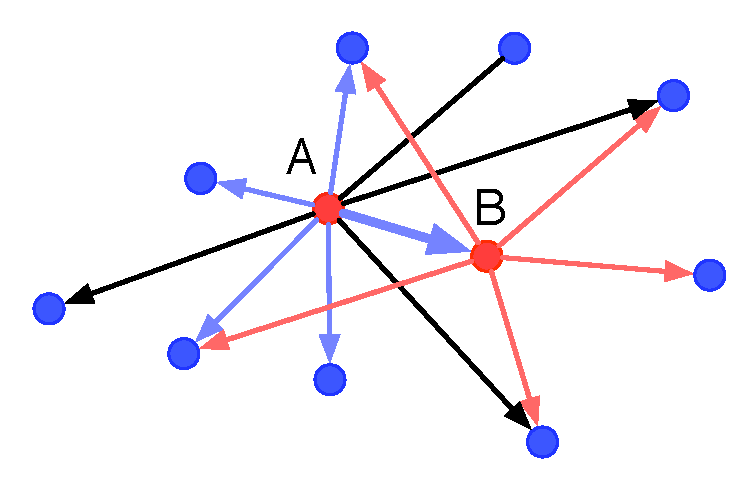
\includegraphics[width=.8\linewidth]{figures/rbf_stencils.pdf}
  \caption{RBFFD Stencils. Each node of the stencil is connected to
    $n_z-1$ stencil nodes in addition to itself. In the figure, node
    $A$ is connected to $B$, but $B$ is {\em not\/} connected to
    $A$. Thus adjacency graph of $A$ is not-symmetric.}
  \label{fig:rbf_stencils}
\end{figure}

Many problems in fluid dynamics and in the geosciences require the
solution to transport equations of the form
\begin{equation}
\pf{Q}{t} = f(Q,\grad{Q},\Laplacian{Q})  \label{eq:Q}
\end{equation}
where $Q$ is a vector of unknowns.
For example, in solving a system of equations, it is
often necessary to compute the derivative of multiple functions along
the same coordinate direction,
typically four for the Euler equations, or five for the Navier-Stokes
equations. Multiple right-hand sides transform a SpMV into a SpMM
(Sparse Matrix/dense Matrix multiplication), which improves register
utilization and decreases cache misses by vectorizing over the
multiple source vectors. Further improvements are possible by
recognizing that different derivative matrices (e.g., gradient and 
Laplacian operators), 
have the same sparsity distribution as long as the derivative stencils
remain unchanged; only the values in the sparse matrix change. 
Thus, rather than computing a derivative of multiple
functions, one can calculate multiple derivatives of a single
function. The increased memory bandwidth due to an increase in the
number of derivative matrices is offset by better cache utilization,
leading to an overall performance benefit. In practice however, the number of 
vectors whose derivatives are required is limited, limiting the 
performance of the matrix/vector multiplication. Similarly, the number
of different derivatives in a particular computation is limited. It is 
for this reason that we seek to combine the benefits of multiple
vectors and multiple matrices simultaneously. We limit this initial 
study to four vectors and four matrices. 


In discrete form, Equation (\ref{eq:Q}) takes the form
$$
  y^{i,j} = A^i x^j 
$$ where $j$ ranges over the number of source vectors, $i$ ranges of
  the number of derivative matrices and there are $i*j$ output vectors
  $y$ (graphically shown in Figure~\ref{fig:struct_comp}).

\begin{figure}
  \centering

  \[ \left( \begin{array}{cccc}
    y^{1,1} & y^{1,2} & y^{1,3} & y^{1,4} \\
    y^{2,1} & y^{2,2} & y^{2,3} & y^{2,4} \\
    y^{3,1} & y^{3,2} & y^{3,3} & y^{3,4} \\
    y^{4,1} & y^{4,2} & y^{4,3} & y^{4,4} 
  \end{array} \right)
  = \left(
  \begin{array}{c}
    A^1\\
    A^2\\
    A^3\\
    A^4
  \end{array}\right)
  \times \left(x^1 x^2 x^3 x^4 \right) \] 
  
  \caption{Structure of the computation.}
  \label{fig:struct_comp}
\end{figure}


\section{Modelization of the Potential Improvements}
\label{sec:model}

We saw in the previous section that one can express the RBF problem as
a multiplication of four matrices by four vectors. We present here an
estimation of the variation on the flop intensity of the computation
and its impact on the expected performance of the
application. Relevant notations are given in Figure~\ref{tab:not}.

\begin{figure}[tbh]
  \begin{center}
    \scalebox{.8}{
      \begin{tabular}{|c|l|}
        %\hline
        %& & \\
        \hline
        $b_i$ & number of bytes per index \\
        $b_x$ & number of bytes per value \\
        $n_z$ & number of nonzeros per row of $A$ \\
        $n_r$ & number of column/rows of $A$ \\
        $n_c$ & total number of nonzeros\\
        $n_v$ & number of {\tt x} vectors \\
        $n_m$ & number of matrices \\
        $s_M$ & size of the $n_m$ matrices in bytes\\
        $s_x$ & size of the $n_v$ {\tt x} vectors in bytes\\
        $s_y$ & size of the $n_v n_m$ {\tt y} vectors in bytes\\
        \hline
        $cl$    & size of a cache line in bytes\\
        $b_{wT}$ & number of bytes written to memory  \\
        $b_{rT}$ & minimum number of bytes read from memory  \\
        $b_T$   & minimum number of bytes transferred \\
        $B_{rT}$ & maximum number of bytes read from memory \\
        $B_T$   & maximum number of bytes transferred \\
        $O$     & number of floating point operations \\
        $I_b$   & maximum computational intensity\\
        $I_w$   & minimum computational intensity\\        
        \hline
      \end{tabular}
    }
  \end{center}
  \caption{Notation relative to the application problem (upper section) and to the benchmarks (lower section.)}
  \label{tab:not}
\end{figure}

Each vector in the problem is of dimension $n_r$ and each entry
takes $b_x$ bytes. There are $n_v$ {\tt x} vectors and $n_v n_m$ {\tt
  y} vectors, which lead to the size of the {\tt x} and {\tt y} vectors:
$$s_x = n_v b_x n_r$$ $$s_y = n_v n_m b_x n_r$$

The matrix is composed of $n_r$ rows and columns with $n_z$ nonzeros
per row leading to a total of $$n_c = n_r n_z$$ nonzero entries in
the matrix. Each of these nonzero entries has one index of size $b_i$
and $n_m$ values of size $b_x$. The matrices have a total size
of $$s_M = n_c (b_i + b_x n_m) = n_r n_z (b_i + b_x n_m)$$

\begin{figure*}[tbh]
  \centering
  \subfigure[Best case.]{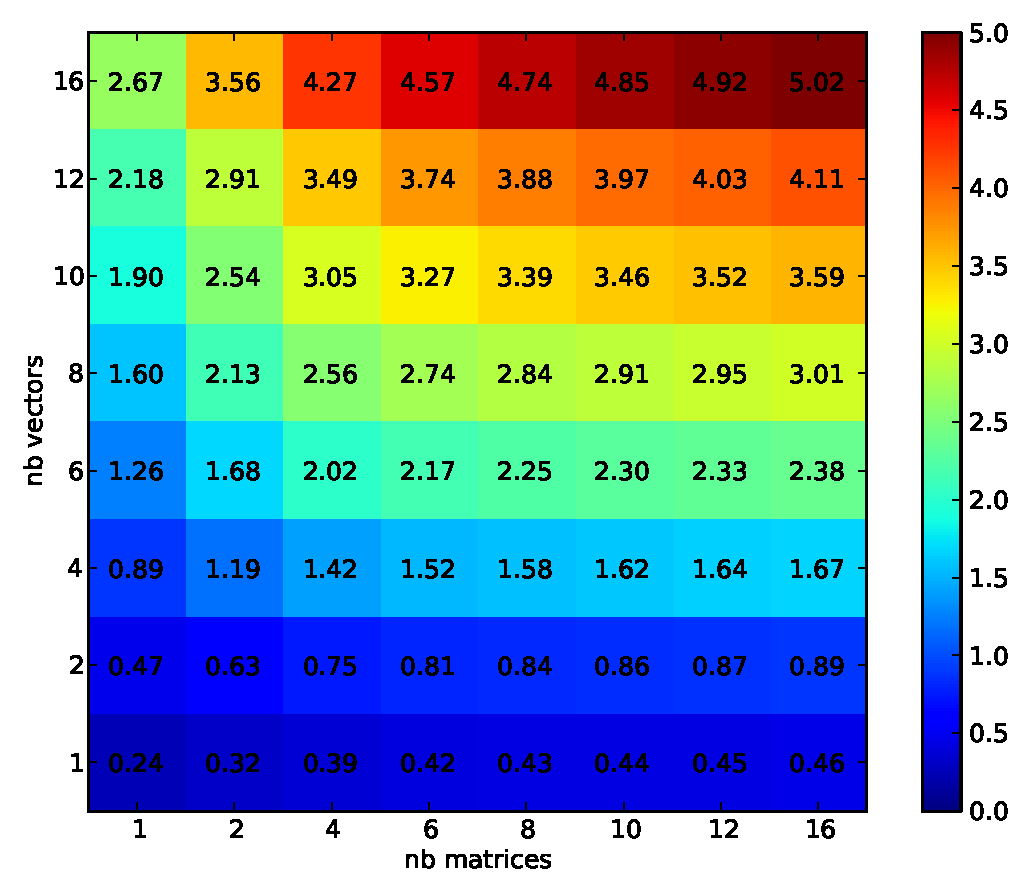
\includegraphics[width=.33\linewidth]{figures/flops_to_bytes_best-crop.pdf}\label{fig:ratio_best}}%
  \subfigure[Worst case.]{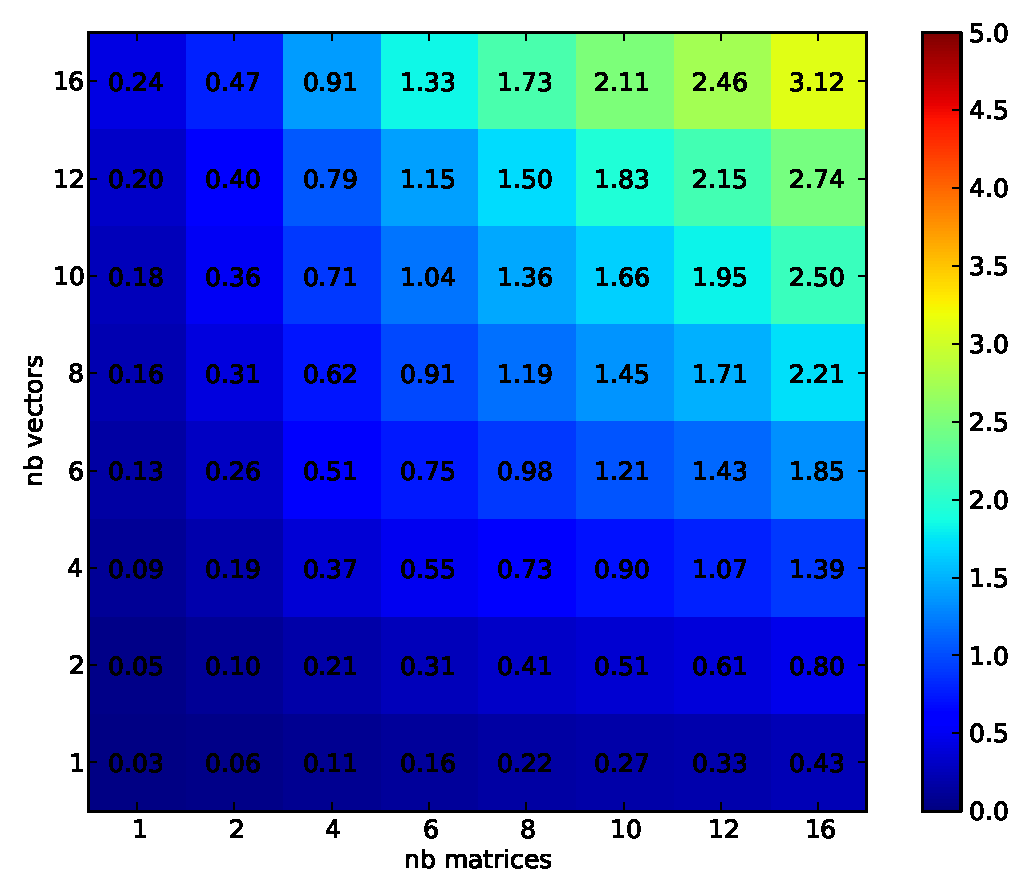
\includegraphics[width=.33\linewidth]{figures/flops_to_bytes_worst-crop.pdf}\label{fig:ratio_worst}}%
  \subfigure[Worst case (No cacheline effects)]{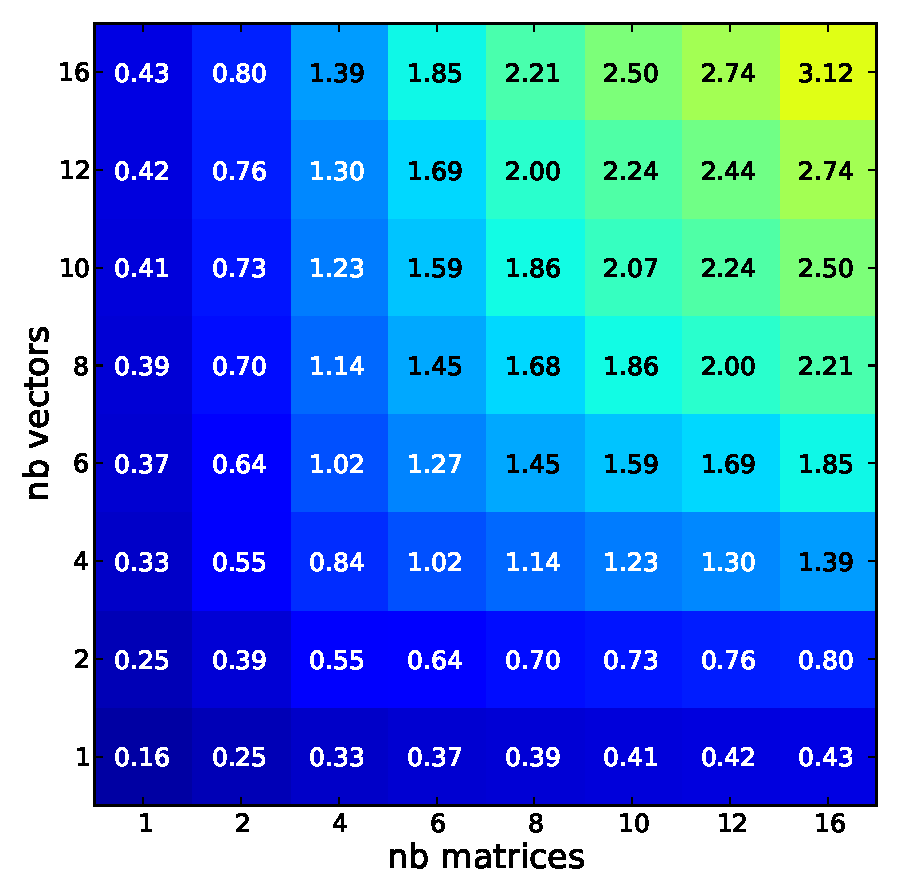
\includegraphics[width=.33\linewidth]{figures/flops_to_bytes_no_cache-crop.pdf}\label{fig:ratio_worst_nocache}}
  
  \caption{Ratio of flops to bytes in single precision:  
    \ref{fig:ratio_best} best case; \ref{fig:ratio_worst} worst case when $cl=64$ 
    ; and \ref{fig:ratio_worst_nocache} worst case neglecting that the
    memory transfers are with a granularity of one cache line (equivalent to $cl = 1$)}
  \label{fig:ratio_bytes_flops}
\end{figure*}


If we assume an algorithm where the rows are processed one after
the other, the amount of memory written is precisely the
size of the {\tt y} vector. (This assumption removes the possibility of
blocking or cache partitioning techniques.) $$b_{wT} = s_y = n_v n_m b_x n_r$$

The amount of data read from memory depends highly on both the
algorithm's execution path, and on how the matrix is structured. But
in the best case both the matrix $A$ and the source vector {\tt x} are
read once from the main memory. (We assume that all the elements of
$\tt x$ are involved in the SpMV.)  Thus, $$b_{rT} = s_M + s_x = n_r
n_z (b_i + b_x n_m) + n_v b_x n_r$$
 $$b_T = b_{rT} + b_{wT} =  n_r n_z (b_i + b_x n_m) + n_v b_x n_r (1 + n_m)$$

Notice that there is no reason for a piece of the matrix to be read
multiple times. But assuming that each element of the {\tt x} vector
is read a single time is a strong assumption. If using a single core,
it assumes that either the cache of the architecture can store the full
{\tt x} vector or that the matrix is sufficiently well structured 
to cause no cache trashing. If using multiple cores, this assumes that
no element of the {\tt x} vectors will be used by multiple
cores. \cite{Saule13-ARXIV} showed that there is very little cache trashing
in practice, but it showed that having elements of the vectors used by
multiple cores can have a significant impact on the performance
(growing with $n_v$).

On the other hand, in the worst case, every time the {\tt x} vector is
accessed, the value needs to be transfered from memory again. So in
total, there are as many transfers as the number of nonzeros in the
matrix. Note however that most architectures cannot read memory a
single byte at a time. Instead, a minimum number of bytes, equal to
the size of a cacheline $cl$, are transfered at once.  When there are
multiple vectors, each nonzero element uses $n_v$ consecutive
entries. In the worst case, the number of bytes read and transfered is
$$B_{rT} = s_M + n_c cl \ceil{\frac{n_vb_x}{cl}} $$ 
$$B_T = n_v n_m b_x n_r + n_r n_z \left ( b_i + b_x n_m +  cl \ceil{\frac{n_vb_x}{cl}} \right)$$

In SpMV, each nonzero of the matrix requires two floating point
operations: one for performing the multiplication and one for
accumulating the result row-wise. Here we are dealing with $n_v n_m$
simultaneous SpMVs and the number of floating point operations is
$$O = 2 n_v n_m n_c = 2 n_v n_m n_z n_r$$

The computation intensity is the amount of floating point operations performed per
byte transfered. In the worst case and in the best case, we have
$$I_b = \frac{O}{b_T} = \frac{2 n_v n_m}{ (b_i + b_x n_m) + n_v n_m b_x n_z^{-1} + n_v b_x n_z^{-1} }$$
%$$I_w = \frac{O}{B_T} = \frac{2 n_v n_m}{n_v n_m b_x n_z^{-1} + \left ( b_i + b_x n_m +  cl \ceil{\frac{n_vb_x}{cl}} \right)}$$
$$I_w = \frac{O}{B_T} = \frac{2 n_v n_m}{(b_i+b_x n_m) + n_v n_m b_x n_z^{-1} + cl \ceil{\frac{n_vb_x}{cl}} }$$


Figure~\ref{fig:ratio_bytes_flops} presents the flop to byte ratios
for single precision computation in the best and the worst case on a
classical cache based architecture ($cl = 64$) and assuming $cl=1$. We
can easily see the potential improvement in the computational
intensity when the number of matrices or vectors increases. There is a
significant difference between the best and the worst case: there is a
eightfold difference in the one matrix -- one vector ($n_m=n_v=1$) case but that gap closes
with the increase in the number of vectors and matrices to a fourfold
difference in the four matrices and four vectors ($n_m=n_v=4$) case and 1.6 fold in the 
$n_m=n_v=16$ case. 
The ratios computed with $cl = 1$ are mostly
similar to the one with $cl=64$ when the number of vectors is
large. But the differences are important when the number of vectors is
low: this highlights that accessing the memory with a granularity of one cache
line
is the main problem faced when performing a standard SpMV computation.

Figure~\ref{fig:perf_predict} shows how these ratios translate
into actual performance. This figure provides projected best and worst
Gflop/s achievable assuming the computation is memory-bound and the
architecture reaches 150~GB/s. Notice that \cite{Saule13-ARXIV}
showed a higher peak bandwidth, but we will show in
Section~\ref{sec:expe} why 150~GB/s is a better estimate of what one
might achieve in these kernels. In single precision, the worse that
one could achieve by using four vectors and four matrices is much higher
than the best achievable using a classical SpMV computation. The best
performance reachable is 210~Gflop/s: almost six times higher than the
peak of the classical SpMV case. 


\begin{figure}
  \centering 
  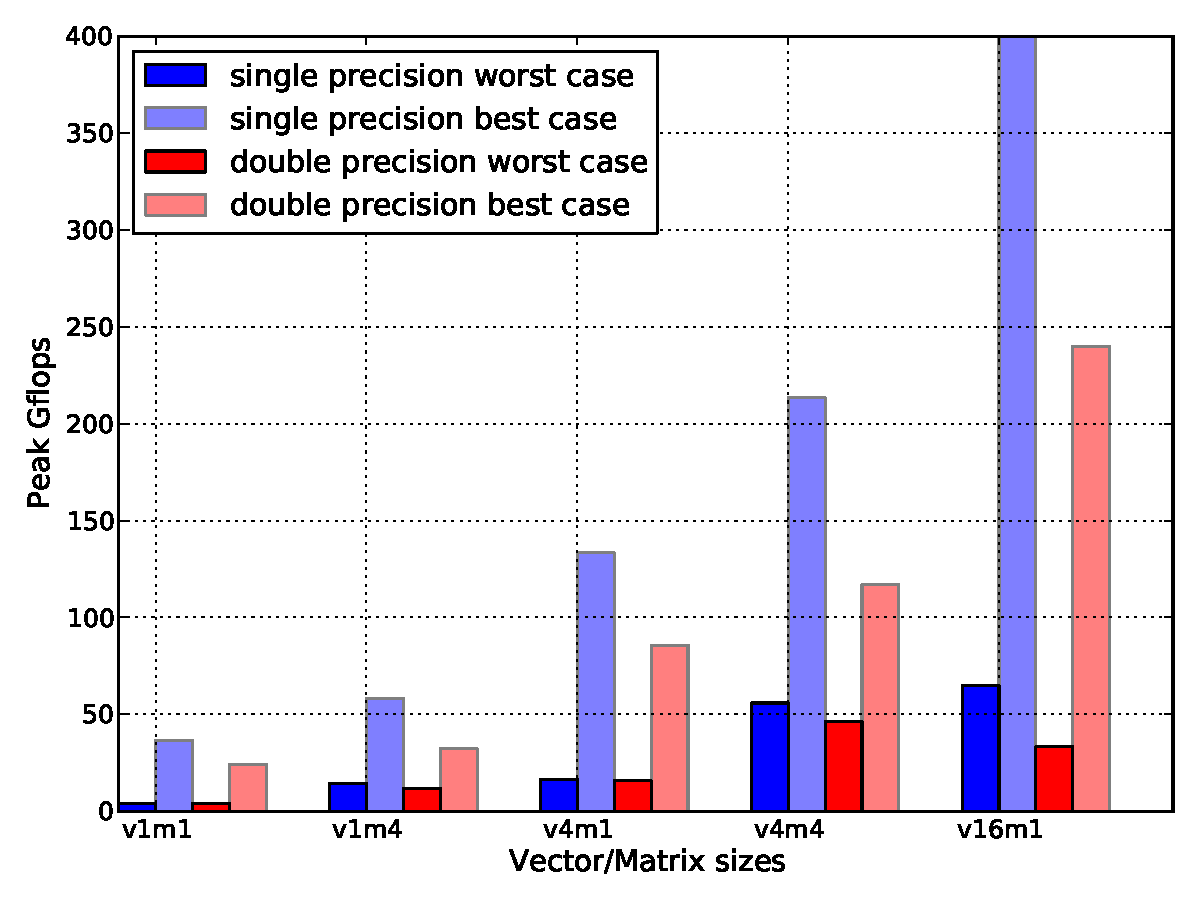
\includegraphics[width=.9\linewidth]{figures/gflops_peak.pdf}\label{fig:gflops-peak-perf}
  \caption{Estimation of the maximum achievable performance using a
    device with a bandwidth from memory to computational units of 150~GB/s when
    varying the number of vectors and matrices.}
  \label{fig:perf_predict}
\end{figure}

\section{Efficient Implementation on the Intel Xeon Phi processor}
\label{sec:impl}

\subsection{Knights Corner}

In this work, we use an Intel Xeon Phi 5110P coprocessor. This card
has 8 memory controllers that can each execute 5 billion
transactions per second. Each has two 32-bit channels, achieving a total
bandwidth of 320~GB/s aggregated across all the memory
controllers. There are 60 cores clocked at 1.05~GHz. Their memory
interfaces are 32-bit wide with two channels and the total bandwidth
is 8.4~GB/s per core. Thus, the cores should be able to consume 504~GB/s
at most. However, the bandwidth between the cores and the memory
controllers is limited by the ring network that connects the cores and
the memory controller. Its precise bandwidth is unknown but it is
believed to be between 200~GB/s and 250~GB/s.

Each core in the architecture has a 32kB L1 data cache, a 32kB L1
instruction cache, and a 512kB L2 cache. The architecture of a core is
based on the traditional Pentium architecture, which has been extended to
64-bit. A core can hold four hardware contexts at any given time. At each
clock cycle, instructions from a single thread are executed. Due to
some hardware constraints, two hardware contexts must be used to reach
the peak instruction throughput in that architecture. Similar to the
Pentium architecture, a core has two different concurrent instruction
pipelines that allow the execution of two instructions per
cycle. However, only one vector or floating point instruction can be
executed at each cycle.

Most of the performance of the architecture comes from the vector
processing unit. Each core has 32 512-bit SIMD registers that can be
used for double or single precision, that is, either as a vector of 8
64-bit values or as a vector of 16 32-bit values, respectively. The
vector processing unit can perform many basic instructions, such as
addition or division, and mathematical operations, such as {\tt sin} and
{\tt sqrt}, making it possible to reach 16 single precision (or 8 double precision)
operations per cycle.  
The unit also supports Fused Multiply-Add (FMA)
operations, which are typically counted as two operations for
when benchmarking. Therefore, the peak performance of the 5110P
card is 1 Tflop/s in double precision and 2 Tflop/s in single
precision. If FMA cannot be used, only half of these rates can be
achieved.


\subsection{Bringing the data into the vector register}

As explained in Section~\ref{sec:model}, we expect to achieve a performance of
about 210~Gflop/s in single precision in the best case. We will focus
on the single precision case with four vectors and four matrices. 
Similar techniques apply for other matrix/vector combinations. This target
performance represents 10\% of the peak performance of the
architecture which is impossible to reach without an efficient vectorization of
the kernel. Indeed, to reach such a performance, a Fused Multiply-Add
instruction on fully loaded registers must be executed at most every
10 cycles.

In term of memory layout, we adopt a format similar to the ELLPACK
format to store the matrix since the number of nonzeros per row is
constant throughout the matrix. The matrix is given in two arrays. The
first one is the classical {\tt col\_id} array that describes the
sparsity structure of the matrix. Each row of {\tt col\_id} consists
of $n_z$ entries that label the column index of each nonzero in
$A$. The other array is the {\tt data} array that gives the values of
the nonzeros in the four matrices. The values of the matrices are
interleaved by groups of four so that the value $A^l_{col\_id[k]}$ of
the $k$th nonzero of the $l$th matrix is at index $\floor{\frac{k-1}{4}}*4*n_m + (l-1)*4+(k-1)\%4$.
(In other words, the first 4 entries are from $A^{1}$ and the next 4 are from $A^2$.) The vectors {\tt x} are
interleaved so that {\tt x}$^l_i$ and {\tt x}$^{l+1}_i$ are
consecutive in memory. The vector {\tt y} is similarly interleaved,
grouped in sets of 16, which correspond to four derivatives applied to
four functions, at a single point.


We discuss how the implementation of the v4m4 kernel works using
vectorial instructions. The code is given for reference in
Figure~\ref{code:mat_mul}. (We will show in Section~\ref{sec:expe}
that an implementation that relies on compiler vectorization does not lead
to desirable performance, which confirms the results
of~\cite{Saule13-ARXIV}.) The registers in the MIC architecture are
512 bits wide and can store 16 floats or integers. (In comparison to
OpenCL or CUDA, one can think of these registers as a warp.) The end
goal is to load and format the nonzero values $A_h^1,A_h^2,A_h^3,A_h^4$
and the vector entries $x_m^1,x_m^2,x_m^3,x_m^4$ in two vector registers and 
apply Fused Multiply-Add on them, which is depicted in the {\tt accu} line of 
Figure~\ref{code:mat_mul}. Bringing the data into the vector
register as depicted in the figure is the difficult component of our 
proposed algorith, which we proceed to explain further. 
A thread will perform the multiplications one row at a time,
and parallelism is achieved by giving blocks of rows to each core
using an OpenMP construct.

\begin{figure*}
  \centering
\subfigure[Source code]{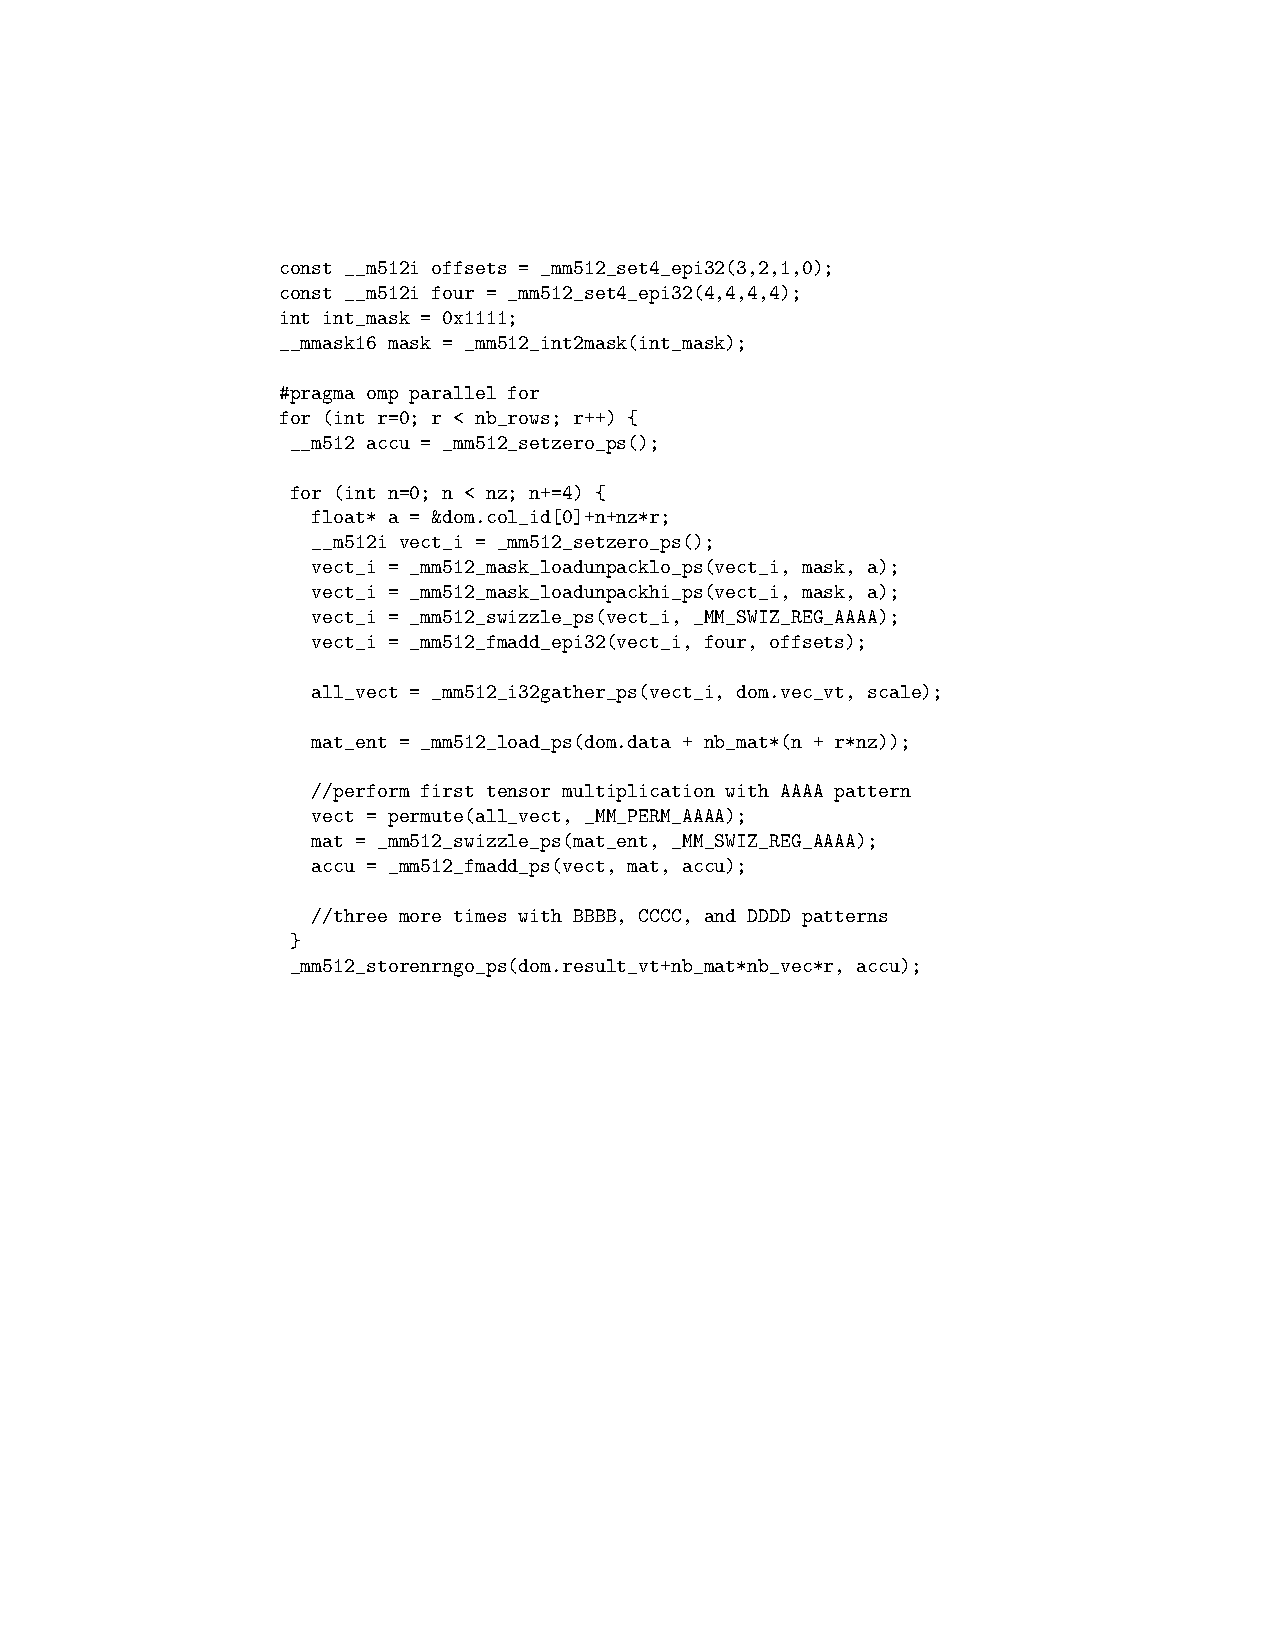
\includegraphics[clip=true,trim=4.5cm 11cm 4cm 4.2cm,width=.6\linewidth]{code.pdf}}%
\subfigure[Content of the vector registers]{\hspace{-0.07\linewidth}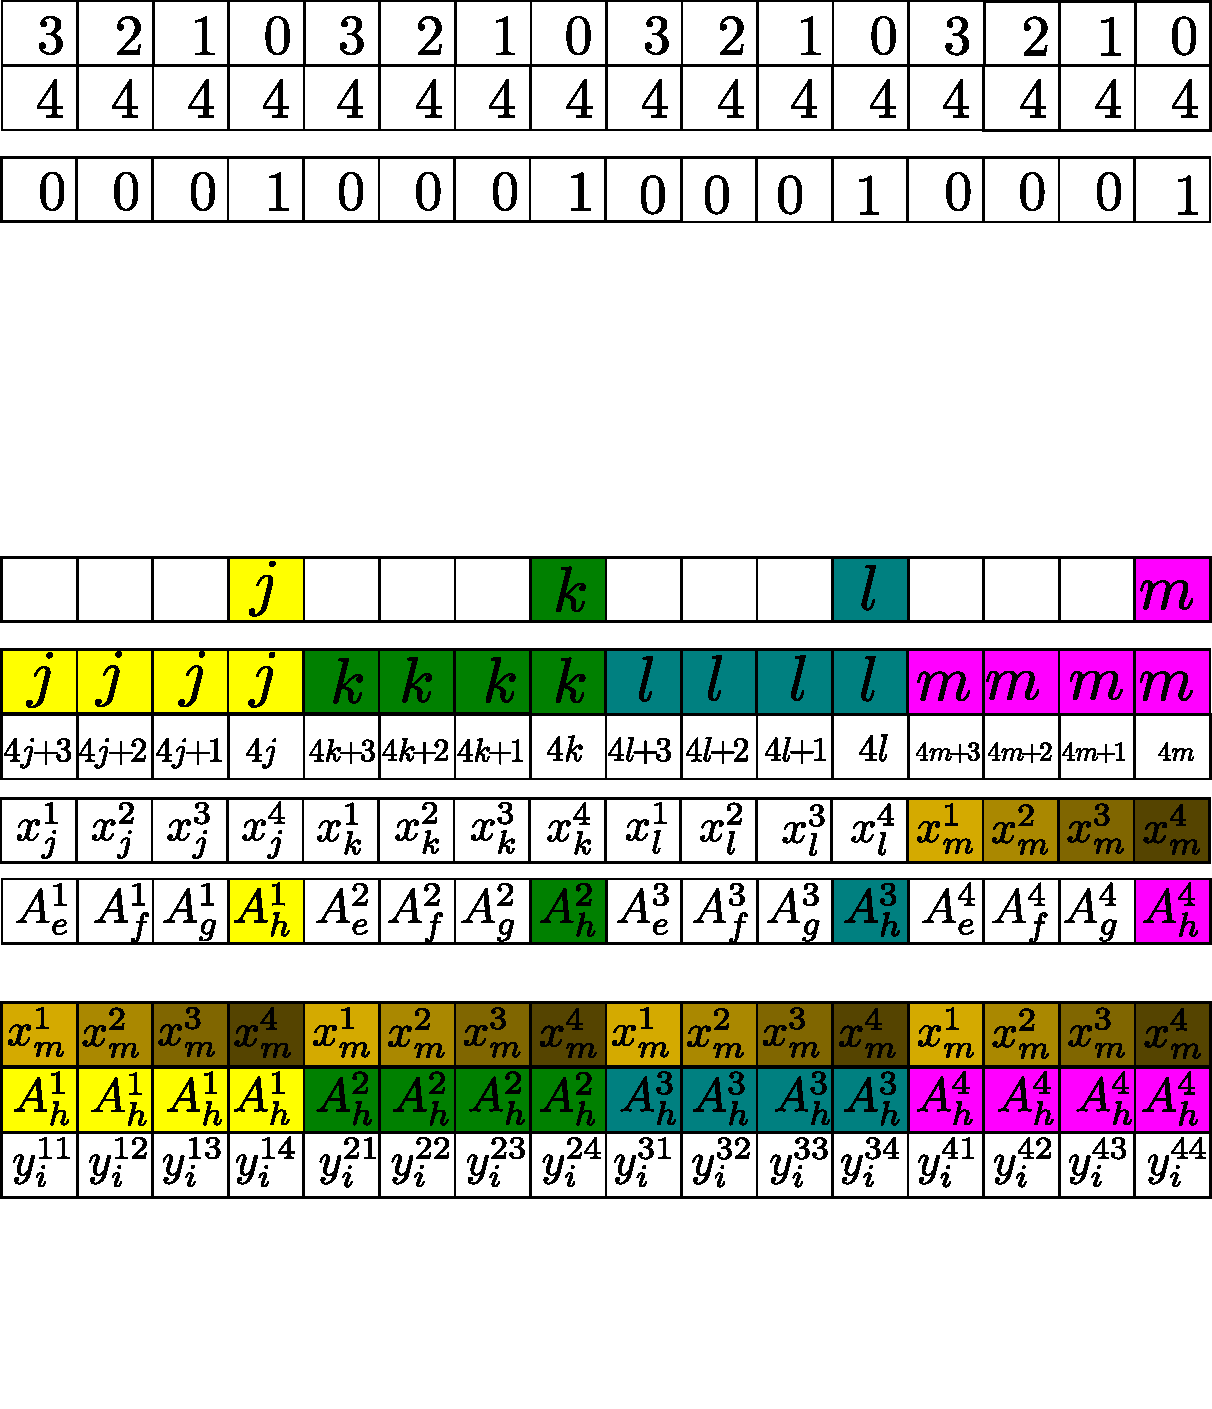
\includegraphics[width=.5\linewidth]{figures/code-annote.pdf}}

\caption{Code snippet of the multiplication of 4 vectors with 4
  matrices. When a line changes the content of a vector register its
  new content is shown on the right. The effects of swizzling and
  permutations are highlighted using a color code.}
\label{code:mat_mul}
\end{figure*}


The core of the technique is the use of swizzling and permutation
features of the vectors in the Intel MIC architecture. A vector of 512
bits is composed of four lanes (sometimes called channels) of 128
bits, which are made of four segments of 32 bits. A swizzling
operation allows the reorder of the elements within each lane (see how
{\tt mat} is extracted from {\tt mat\_ent} in
Figure~\ref{code:mat_mul}). While a permutation reorders entire lanes,
without changing their contents (see for instance how {\tt vect} is
generated from {\tt all\_vect} in Figure~\ref{code:mat_mul}).  Both
permutation and swizzling support common reordering and broadcast. In
the code, the ``permute'' function needs to use the {\tt
  \_mm512\_permute4f128\_epi32} instruction which is only defined on
integers and therefore in place typecasts are necessary to convert to
a vector to/from the integer type.  (Note that we prefer swizzling to
permutation if possible because we believe it is cheaper. Many
instructions have swizzling capability, while permuation is its own
instruction. %\todo{do we need a reference to intel Xeon phi instruction set?})

Every operation that loads data from memory into a register
transfers 512 bits, or 16 floats at a time. A single nonzero
in the matrix will cause 16 operations to be performed, but it only
uses 4 floats from the matrix and 4 floats from the {\tt x} vector. So
we would like to execute a single instruction to load the data for four 
nonzeros in the matrix, and another instruction to load the data for
four nonzeros from the vectors.  
%representing 16 floats from the matrix and 16 floats from the vectors at once. 
(The number of nonzeros on a row in our application is
always a multiple of 4; if it weren't, we would add some explicit
zeroes in the data structure for padding.)
\todo{Erik, I rewrote the paragraph. Please reread.}

The values from the nonzero elements in the matrix are the simplest to
load. One can load the 16 floating point values for four nonzeroes of
the matrix at once. The four floats coming from each matrix are
naturally grouped within each lane of the SIMD vector. One can use a
swizzle operation to broadcast the 4 elements of a single matrix to
take the whole vector. (The broadcast of $A_h^1,A_h^2,A_h^3,A_h^4$ is
shown in Figure~\ref{code:mat_mul}.)

Loading the entries from the {\tt x} vector is a little bit more
involved. First, the columns pointers of four different nonzeros are
loaded into a vector register and the values are distributed one per
lane of the vector register using an {\tt unpack}
operation\footnote{Notice that there are two calls to unpack for the
  LSB and MSB. Both are mandatory even if one is known not to be
  useful according the documentation of the hardware}. (The column
pointers are named $j,k,l,m$ in Figure~\ref{code:mat_mul}.) They
are replicated so that each value fills an single vector lane 
using a swizzle operation. Then each value is multiplied by 4 
(because there are 4 vectors) 
and the offset vector $(3,2,1,0)$ is added to each lane to obtain the
correct index of the elements of the {\tt x} vector within each lane
using a Fused Multiply-Add operation. Then a {\tt gather} operation is
performed to bring the 16 entries of the {\tt x} vector into the SIMD
register. At this point we have a SIMD register where each lane is the
four vector entries for a nonzero element. Using a broadcast
permutation, one can replicate an entry of the four vectors across
each lane. (The broadcast of $x_m^1,x_m^2,x_m^3,x_m^4$ is shown in
Figure~\ref{code:mat_mul}.)

Now that $A_h^1,A_h^2,A_h^3,A_h^4$ and $x_m^1,x_m^2,x_m^3,x_m^4$ are
properly laid out in the vectors, a partial value for $y_i$ can be
computed. Once all the nonzeros of the row have been processed, the
exact $y_i$ value can be sent to memory using a the No Read No Global
Order hint to optimize write traffic on the memory bus.


\section{Experimental Validation}
\label{sec:expe}
In this section, we describe a series of numerical experiments to
confirm the performance predictions of Section~\ref{sec:model}. To
better understand our results, we first perform some bandwidth
measurements, followed by the actual SpMV computations. All the codes
are compiled with the Intel C Compiler version 13 and
-O3 optimization. The MIC codes use the IMCI instructions exposed by
the compiler through intrinsics.

\subsection{Bandwidth}

\begin{figure}[bth]
  \centering
  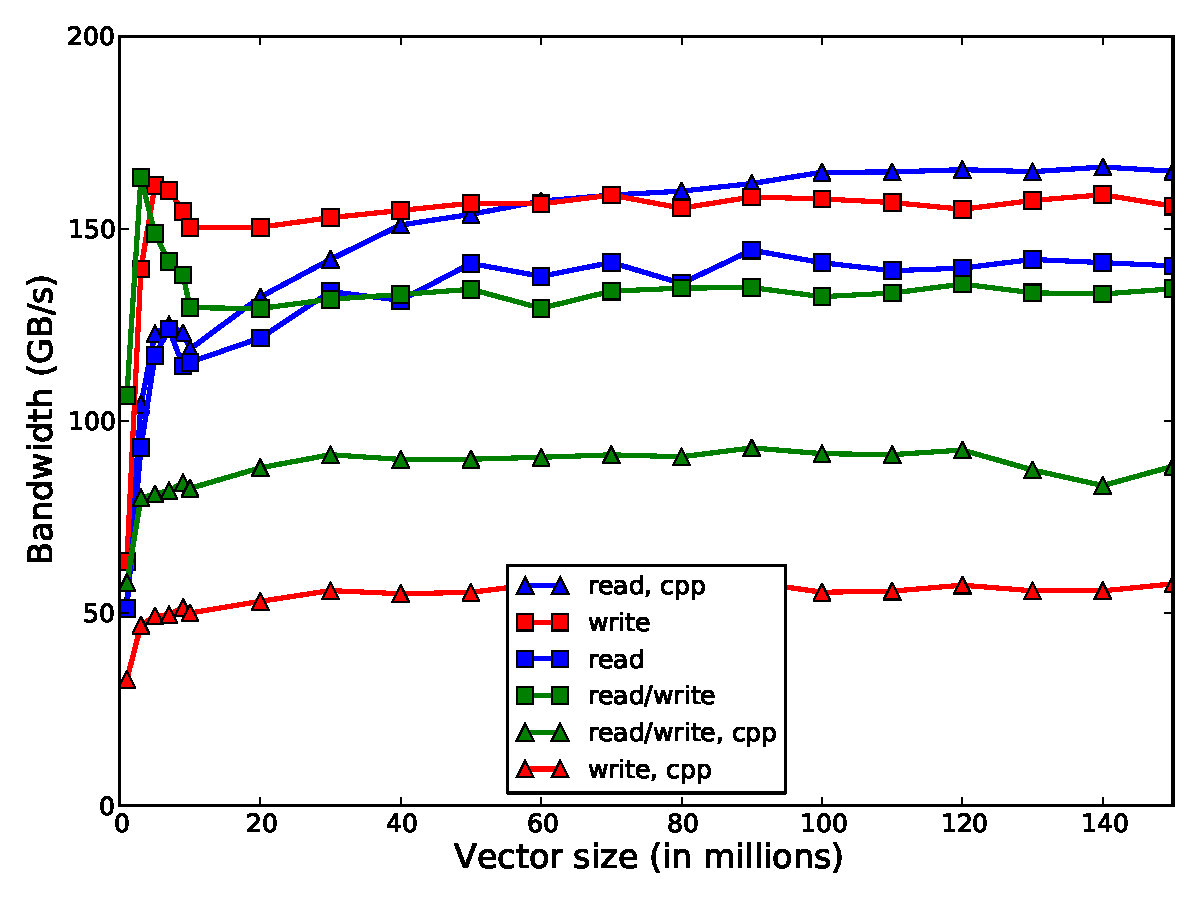
\includegraphics[width=.9\linewidth]{figures/bandwidth_read_write.pdf}
  
  \caption{Bandwidth performance under idealized conditions.  Entries
    with "cpp" (triangles) denote cases where vectorization is
    compiler generated.}
  \label{fig:bandwidth}
  \label{fig:band_rw_MIC}
\end{figure}

Figure~\ref{fig:bandwidth} gives some benchmark that computes the
bandwidth achieved when reading and/or writing large arrays on both
the MIC card and the CPU architecture. The read benchmark performs a
simple sum of the array. The write benchmark sets all the elemnts of
the array to zero, while the read/write benchmarks copies the array into
another one. We also investigate the difference between a straight C++
implementation (compiled with -O3 with proper tagging to inform the
compiler of memory alignments) and a simple implementation with
explicit use of the vector registers.

When using the MIC card (Figure~\ref{fig:band_rw_MIC}), the {\tt
  read\_cpp} implementation reaches a performance of 168~GB/s
 which is better than the {\tt read}
implementation which only achieves 145~GB/s. This
is explained by the compiler adding loop unrolling and software
prefetching in the assembly code in the {\tt read\_cpp} case, which is
not added in the {\tt read} case. On the other hand, the {\tt write}
case reaches a performance of 158~GB/s while the
{\tt write\_cpp} implementation never exceeds 58~GB/s. 
This difference is due to the use of the {\tt \_mm512\_store\_nrngo\_ps} instruction, 
which bypasses the Read For Ownership protocol and allows the writes
to be performed in any order. The compiler can not use this
instruction on its own because this would break the memory convention
useful for some parallel algorithms. The {\tt read/write} benchmark
performs at 140~GB/s while the {\tt read/write cpp} benchmark performs
at about 90~GB/s.

Note that SpMV kernels will likely use only simple read and simple
writes on the MIC architecture. We also benchmark the performance we
can achieve using {\tt gather} and {\tt unpack} operations and we
present the results in Figure~\ref{fig:band_gather}. The {\tt unpack}
instruction can reach a performance of 140~GB/s. (There is no easy way
to implement the equivalent of the {\tt unpack} operation without
using explicit registers.) The performance of the {\tt gather}
operations depends in which order the array is read. If the indices
are ordered ({\tt compact}) then a performance of 140~GB/s is
reached. If the indices are completely randomized, the performance
drops below 5~GB/s. We can see that implementing the
indirection mechanism without vector instructions lowers the
performance significantly. (In the {\tt compact} case, it never
surpasses 100~GB/s and is close to 50~GB/s most of the time.)

\begin{figure}
  \centering
  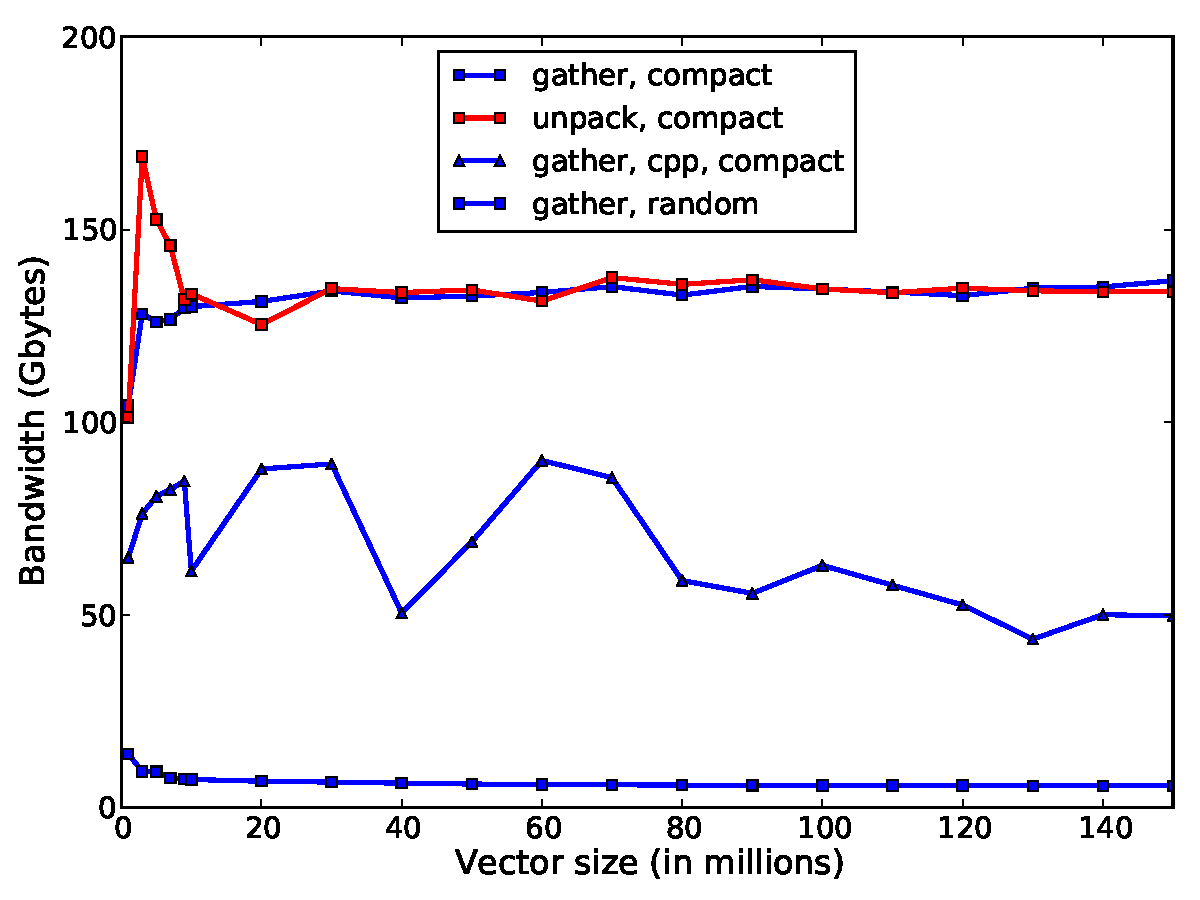
\includegraphics[width=.9\linewidth]{figures/bandwidth_gather_unpack.pdf}
  \caption{Performance of {\tt gather} and {\tt unpack} operations.}
  \label{fig:band_gather} 
\end{figure}
%

To summarize, using vector instructions appears necessary in order
toreach the highest bandwidth on the MIC architecture. For the instructions used
in a typical SpMV computation, one can expect a bandwidth between
140~GB/s to 160~GB/s. That is why we use in our estimations a best
achievable bandwidth of 150~GB/s despite the fact that a 
carefully crafted code to maximize bandwidth can reach higher
values~\cite{Saule13-ARXIV}. 

\subsection{Instances}

\def\ww{.19\textwidth}
\begin{figure*}[tbh]
  \begin{center}
    \subfigure[Supercompact.]{%
      \label{fig:supercompact}
      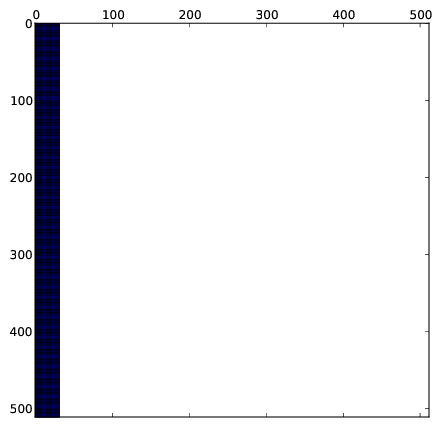
\includegraphics[width=\ww]{figures/supercompact_matrix-crop.png}}%
    \subfigure[Compact.]{%
      \label{fig:compact}
      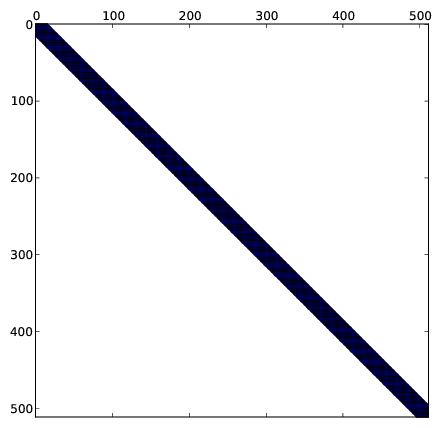
\includegraphics[width=\ww]{figures/compact_matrix-crop.png}}%
    \subfigure[Random.]{%
      \label{fig:random}
      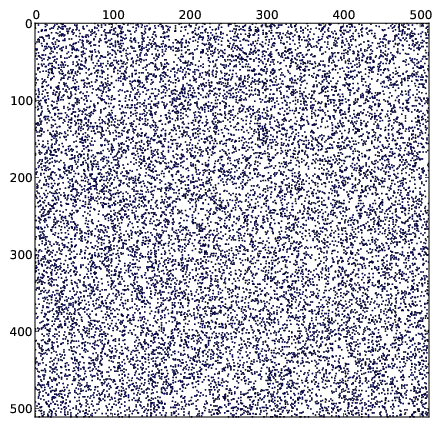
\includegraphics[width=\ww]{figures/random_matrix-crop.png}}%
    %% \subfigure[2D, no RCM.]{%
    %%   \label{fig:rbf2dnorcm}
    %%   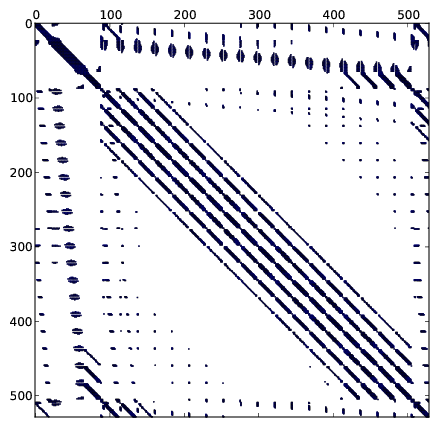
\includegraphics[width=\ww]{figures/kd-tree-2d-norcm-crop.png}}%
    %% \subfigure[2D, RCM.]{%
    %%   \label{fig:rbf2drcm}
    %%   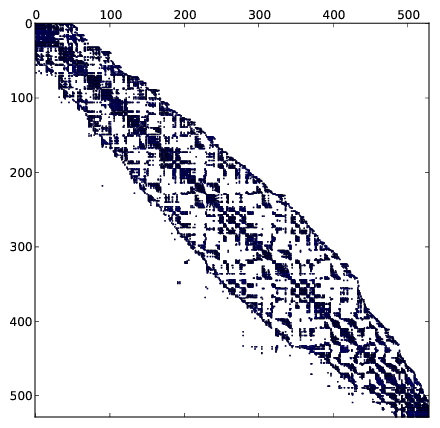
\includegraphics[width=\ww]{figures/kd-tree-2d-rcm-crop.png}} 
    \subfigure[3D, RCM.]{%
      \label{fig:rbf3dnorcm} 
      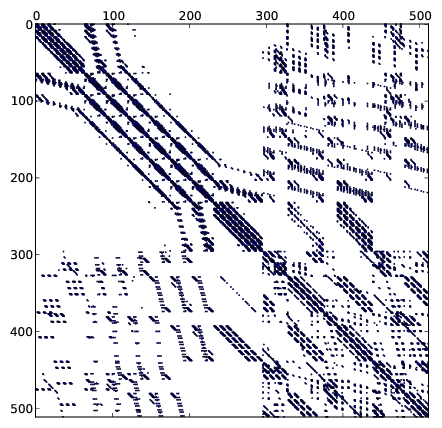
\includegraphics[width=\ww]{figures/kd-tree-3d-norcm-crop.png}}%
    \subfigure[3D, no RCM.]{%
      \label{fig:rbf3drcm}
      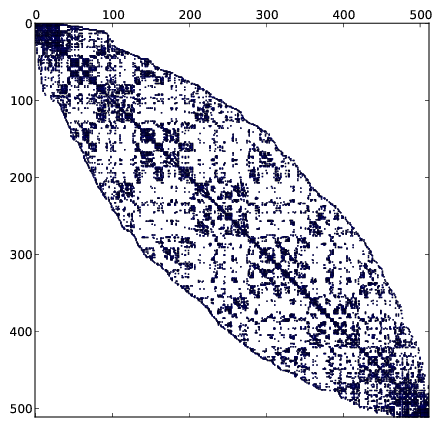
\includegraphics[width=\ww]{figures/kd-tree-3d-rcm-crop.png}}%
  \end{center}
  
  \caption{Different sparsity distributions. In all cases, there are
    512 rows and 32 nonzeros per row. The last two matrices
    corresponds to a derivative stencil in 3D RBF-FD
    calculations (with and without RCM ordering).}
  \label{fig:spy_plots}
\end{figure*}

The different matrices used to perform our experiments and analysis
are presented in Figure~\ref{fig:spy_plots}. The
Supercompact matrices (Figure~\ref{fig:supercompact}) have been
generated to only have nonzero elements in the first 32 columns of
the matrix. As a result, only 32 values of {\tt x} are read
from memory, and the expense associated with cache misses and gather
operations is removed from consideration. The cost associated with 
{\tt A} remains.   \todo{reread the above. Reread by Gordon}
The Compact matrices
(Figure~\ref{fig:compact}) are generated to have 32 nonzeros per row
centered around the diagonal and it represents the ideal case for many
applications that rely on sparse matrix vector multiplication. The nonzero
elements of the Random
matrices (Figure~\ref{fig:compact}) see their nonzero elements
randomly (uniformly) distributed in the matrix; they represent the
worst case scenario for a cache based architecture where the cache
reutilisation is the lowest from one row to the next.

The other two types of matrices are used in derivative stencils in 3D
RBF-FD calculations (Figure~\ref{fig:rbf3dnorcm} shows a $32$-points
stencil of a 3D $8^3$ grid). We also apply a Cuthill-Mckee reordering to
all the matrices.  This ordering technique is designed to reduce the
distance between the nonzeros and the diagonal, hopefully allowing a
better cache reutilisation. The reordered version of the matrix can be
seen in Figure~\ref{fig:rbf3drcm}.


\subsection{Computations}

\begin{figure*}[t]
  \centering
  \subfigure[Supercompact and Random.]{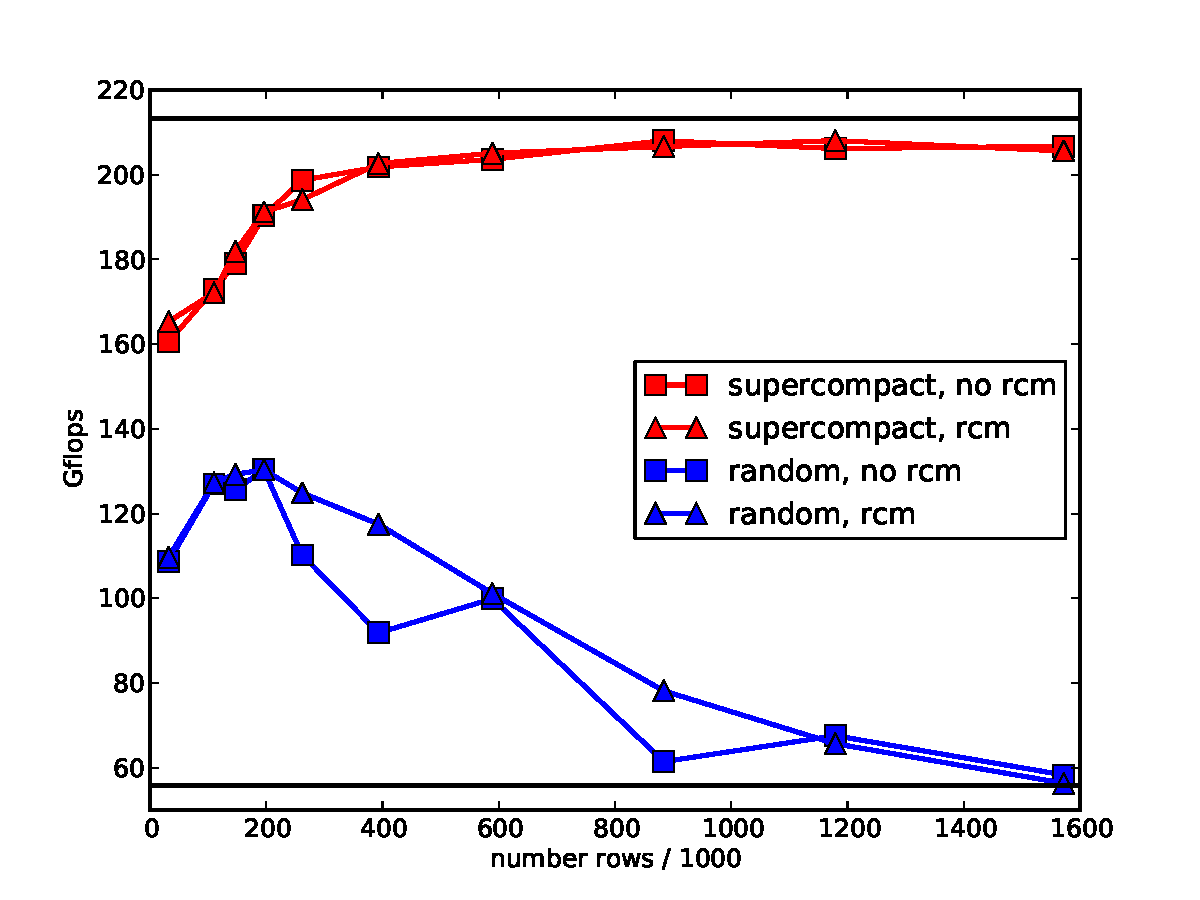
\includegraphics[width=.48\linewidth]{figures/random_supercompact.pdf}\label{fig:perf_ideal}}
  \subfigure[Compact and RBF-FD.]{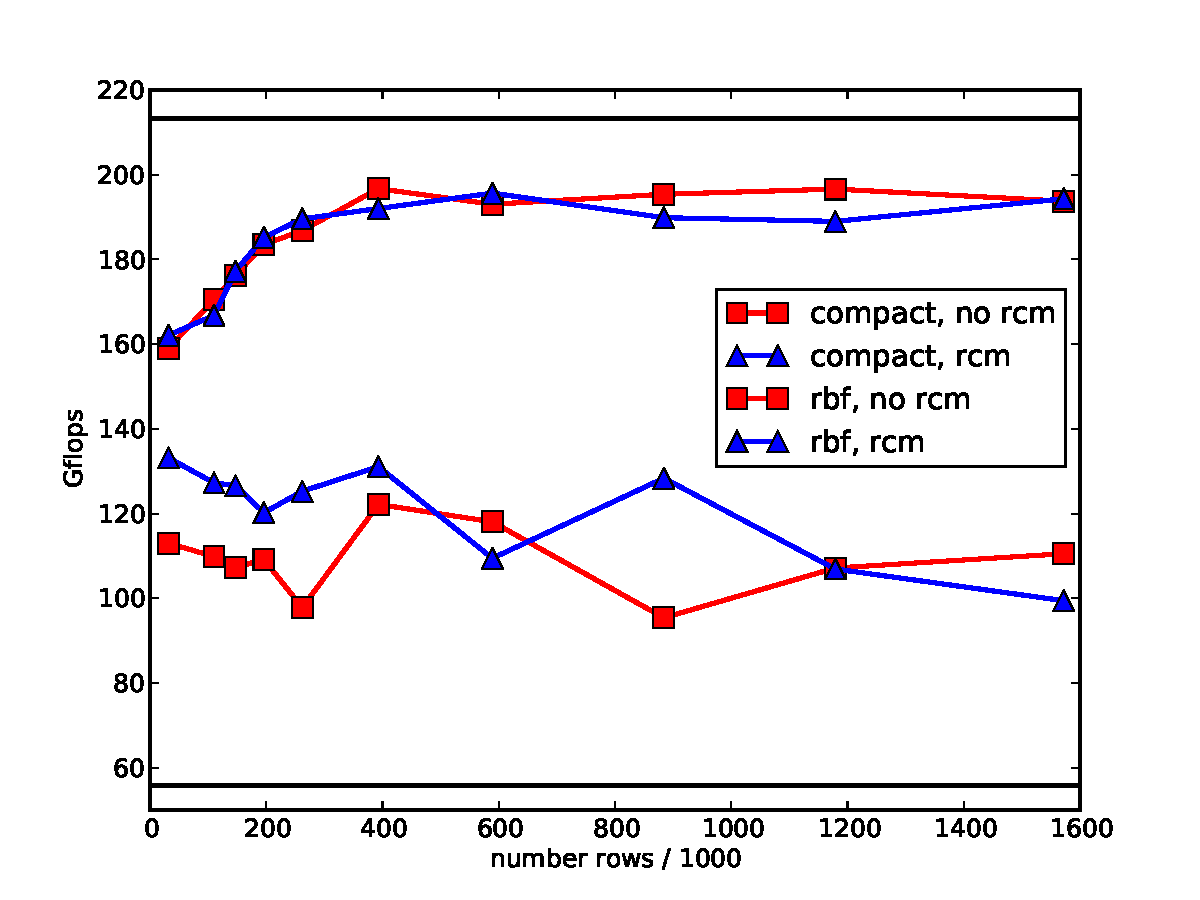
\includegraphics[width=.48\linewidth]{figures/rbf_compact.pdf}\label{fig:perf_realistic}}
  
  \caption{Performance of the manually vectorized code. The two
    horizontal lines depict the worst and the best predicted performances. \todo{font size}}
  \label{fig:expe_types}
\end{figure*}

We now investigate the actual performance that we can obtain when
multiplying four vectors by four matrices in single
precision. Figure~\ref{fig:expe_types} presents results for different
types of matrices and also shows the minimum and maximum performance
predicted in Section~\ref{sec:model}. Figure~\ref{fig:perf_ideal}
gives the results for the {\tt supercompact} and {\tt random} matrices
that represent both the best and the worst case for such a practical 
computation. The {\tt supercompact} case peaks at
208~Gflop/s being very close to the predicted peak
performance of 213~Gflop/s. Conversely the performance of the {\tt
  random} case decreases to 56~Gflop/s which is close to
the lowest predicted performance of 55~Gflop/s. One can see that RCM
ordering helps the {\tt random} case but the impact decreases when the
size of the matrix increases.

Figure~\ref{fig:perf_realistic} gives the results on the {\tt compact}
case, which represents the best realistic matrix one could find with very
structured grids and a
{\tt RBF} derivative matrix extracted from a real 3D application. In the {\tt
  compact} case, the performance can be as high as 195~Gflop/s, which is
within 15\% of the peak predicted performance. The performance of the
{\tt RBF} case varies between 100~Gflop/s and 140~Gflop/s. Most of the
time, the RCM ordering provides an improvement which can be as high as
30~Gflop/s.

\begin{figure}
  \centering 
  
  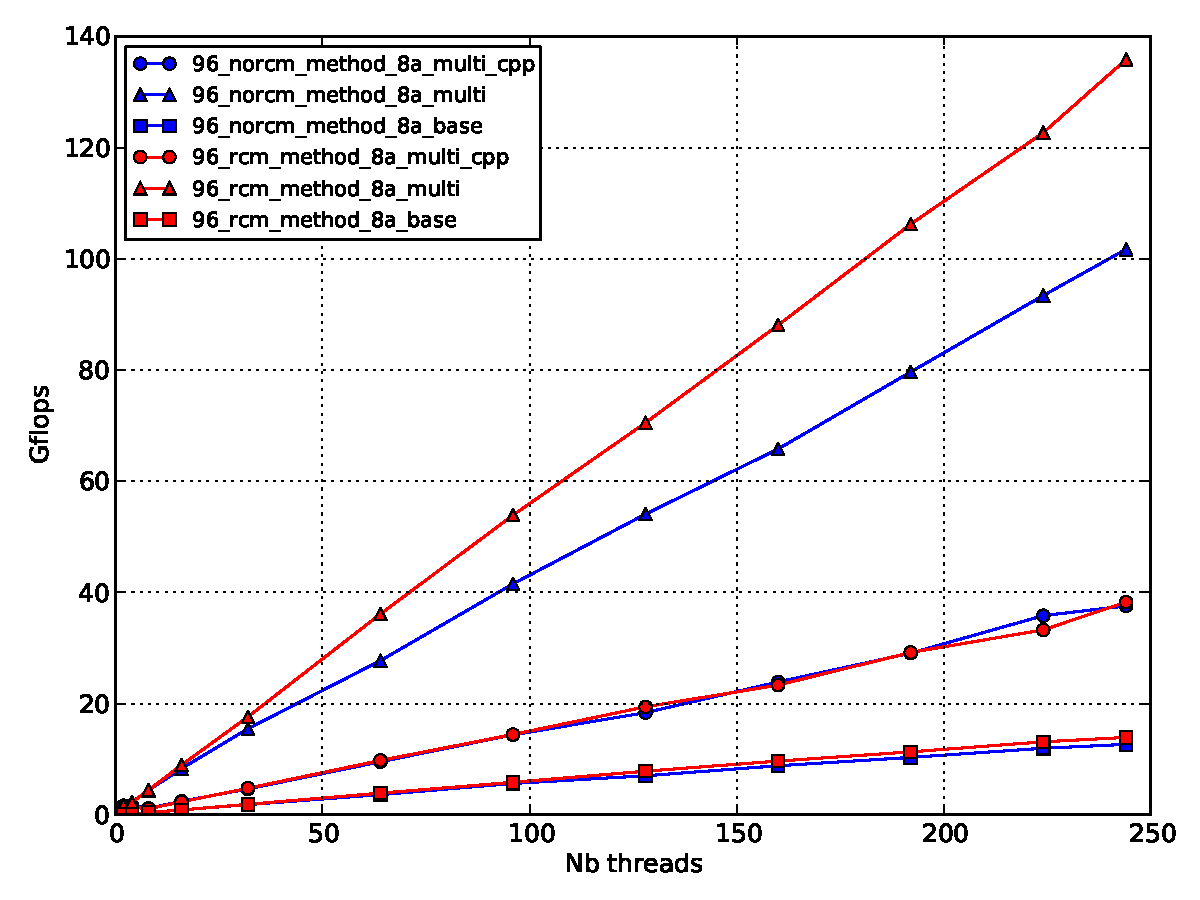
\includegraphics[width=.9\linewidth]{figures/mic_performance_nb_threads.pdf}

  \caption{Performance of $y=Ax$ for a RBF derivative stencil of a
    $96^3$ 3D grid. Classical SpMV ($n_m=n_v=1$ given in blue) has low
    performance. The manually vectorized code (red) is 3.5 times
    faster than the compiler generated one (green). RCM ordering
    (squares) only improves the performance for our manually
    vectorized code.}
  \label{fig:comparison_spmv}
  \label{fig:perf_mic}
\end{figure}

We finally investigate the central questions of this paper. Do we gain
actual performance by transforming classical SpMV computation into the
multiplication of four vectors by four matrices for the computation of the
derivative of RBFs? Does using manual vectorization improve actual
application performance? Figure~\ref{fig:comparison_spmv} compares the
performance achieved by a classical SpMV and by the multiplication of
four vectors by four matrices using either standard C++ code and our
optimized implementation. The
classical SpMV computation reaches 14~Gflop/s. 
The standard C++ implementation reaches a performance of 38~Gflop/s while our
optimized implementation reaches 140~Gflop/s. 
Notice that \todo{I do not know that I ran host and mic on the same grid, but your 
numbers are approximately correct. The numbers are a function of resolution} 
RCM ordering has no impact in the standard C++ implementation while it
provides a significant improvement in our manually vectorized
version. This highlights that the C++ implementation is instruction-bound
while our manually vectorized implementation is most likely 
memory-bound. 

To put things in perspective, we conducted some experiments on a
classical CPU architecture with two Intel Core i7 processors, each has 8
cores that support AVX instructions. Both the compiler-generated and
the manually-written vectorization using AVX instruction reach a
(read) bandwidth of 70~GB/s. This indicates that the performance of
the classical SpMV can not overcome 17~Gflop/s. A generic
implementation of the multiplication of four vectors with four matrices on
the {\tt RBF} matrix reaches a performance of 27~Gflop/s; while a
manual implementation using AVX instruction reaches a performance of
42~Gflop/s. This confirms that our method is sound and generalizes to
architectures than the Intel MIC architecture. \todo{albeit with less 
impressive results given that swizzling is often not available. Swizzling
will become available in a new version of the host: enhanced AVX.}

\section{Conclusion}
\label{sec:ccl}

In the previous sections, we have explored the practical
implementation on a Intel Xeon Phi card of multiple derivative
operators acting on multiple vectors within the context of
RBF-RD. Each derivative has an associated sparse matrix with a fixed
number of nonzeros on each row. While computing a single derivative of
multiple functions is rather common (vectorization occurs over the
vectors), we accelerate the algorithm further by considering multiple
matrices (identical sparsity patterns) acting on multiple vectors. 
We specialize our study to four matrices and four derivatives,
with 16 outputs, computed as a sum of outer products.

Our implementation makes use of the IMCI MIC instruction set and
includes a number of swizzling and channel swapping operations, for an
extremely efficient tensor product implementation. On a $96^3$ 3D
grid, it reaches a performance of 140~Gflop/s which is 2.7 times
faster than the best possible performance achievable for a single
vector and a single derivative and more than 7 times faster than a
practical implementation.

In a future work, we will examine the effect of larger stencil sizes
and double precision. We will also integrate the techniques
presented in this paper within a fluid simulation using RBF-FD.

\section*{Acknowledgment}
The first and last authors acknowledge NSF funding under NSF grant
DMS-\#0934331 (FSU). NCAR is sponsored by the National Science
Foundation. N. Flyer acknowledges support of NSF grant DMS-0934317.


\bibliographystyle{plain} %{IEEEabrv,paper.bib}
\bibliography{paper, bollig}
\end{document}


